% Apresentacao
% ------------------------------------------------------------------------
% ------------------------------------------------------------------------

\title{Monografia TCC}

\documentclass[
	% -- opções da classe memoir --
	12pt,				% tamanho da fonte
	%openright,			% capítulos começam em pág ímpar (insere página vazia caso preciso)
	%twoside,			% para impressão em verso e anverso. Oposto a oneside
    oneside,
	a4paper,			% tamanho do papel. 
	% -- opções da classe abntex2 --
	chapter=TITLE,		% títulos de capítulos convertidos em letras maiúsculas
	%section=TITLE,		% títulos de seções convertidos em letras maiúsculas
	%subsection=TITLE,	% títulos de subseções convertidos em letras maiúsculas
	%subsubsection=TITLE,% títulos de subsubseções convertidos em letras maiúsculas
	% -- opções do pacote babel --    
	english,			% idioma adicional para hifenização
	% french,				% idioma adicional para hifenização
	% spanish,			% idioma adicional para hifenização
	brazil				% o último idioma é o principal do documento    
	]{abntex2}
    
    %\renewcommand{\ABNTEXpartfontsize}{\normalsize}
	%\renewcommand{\ABNTEXchapterfontsize}{ \large}
	%\renewcommand{\ABNTEXsectionfontsize}{\normalsize}
	%\renewcommand{\ABNTEXsubsectionfontsize}{\normalsize}

% ---
% Pacotes básicos 
% ---
\usepackage{lmodern}			% Usa a fonte Latin Modern			
\usepackage[T1]{fontenc}		% Selecao de codigos de fonte.
\usepackage[utf8]{inputenc}		% Codificacao do documento (conversão automática dos acentos)
\usepackage{lastpage}			% Usado pela Ficha catalográfica
\usepackage{indentfirst}		% Indenta o primeiro parágrafo de cada seção.
\usepackage{color}				% Controle das cores
\usepackage{graphicx}			% Inclusão de gráficos
\usepackage{microtype} 			% para melhorias de justificação
\usepackage{todonotes}
\reversemarginpar % Coloca as anotações do lado esquerdo
\usepackage{tabularx}
\renewcommand{\tabularxcolumn}[1]{m{#1}}
\setlength{\marginparwidth}{2.8cm}


\definecolor{algColor}{RGB}{255,206,206} % rgb(255, 206, 206)

% Pacotes para algoritmos/pseudo-código
\usepackage{listings}

\renewcommand{\lstlistingname}{Programa}

\lstset
{ %Formatting for code in appendix
    language=C,
    basicstyle=\footnotesize,
    numbers=left,
    stepnumber=1,
    frame = single,
    showstringspaces=false,
    tabsize=2,
    breaklines=true,
    xleftmargin=10pt,
    breakatwhitespace=false,
    extendedchars=true,
    literate={á}{{\'a}}1 
             {ã}{{\~a}}1
             {é}{{\'e}}1
             {í}{{\'i}}1
             {õ}{{\~o}}1
             {ç}{{\c{c}}}1,
}

\renewcommand{\lstlistlistingname}{Lista de códigos}

% Configura a ``Lista de Códigos'' conforme as regras da ABNT (para abnTeX2)
\begingroup\makeatletter
\let\newcounter\@gobble\let\setcounter\@gobbletwo
  \globaldefs\@ne \let\c@loldepth\@ne
  \newlistof{listings}{lol}{\lstlistlistingname}
  \newlistentry{lstlisting}{lol}{0}
\endgroup

\renewcommand{\cftlstlistingaftersnum}{\hfill--\hfill}

\let\oldlstlistoflistings\lstlistoflistings
\renewcommand{\lstlistoflistings}{%
   \begingroup%
   \let\oldnumberline\numberline%
   \renewcommand{\numberline}{\lstlistingname\space\oldnumberline}%
   \oldlstlistoflistings%
   \endgroup}
% ---
% Pacotes adicionais, usados apenas no âmbito do Modelo Canônico do abnteX2
% ---
\usepackage{lipsum}				% para geração de dummy text
% ---


% ---
% Pacotes de citações
% ---
%\usepackage[brazilian,hyperpageref]{backref}	 % Paginas com as citações na bibl
\usepackage[alf, abnt-etal-cite=2]{abntex2cite}	% Citações padrão ABNT

% --- 
% CONFIGURAÇÕES DE PACOTES
% --- 

\usepackage{abntex_ufrr_dcc}


% PACOTES DE ALGORITMO

\usepackage{algpseudocode,algorithm}
% Declaracoes em Português

\algrenewcommand\algorithmicend{\textbf{FIM}}
\algrenewcommand\algorithmicdo{\textbf{FAÇA}}
\algrenewcommand\algorithmicwhile{\textbf{ENQUANTO}}
\algrenewcommand\algorithmicfor{\textbf{PARA}}
\algrenewcommand\algorithmicforall{\textbf{PARA TODO}}
\algrenewcommand\algorithmicif{\textbf{SE}}
\algrenewcommand\algorithmicthen{\textbf{ENTÃO}}
\algrenewcommand\algorithmicelse{\textbf{SENÃO}}
\algrenewcommand\algorithmicreturn{\textbf{RETORNE}}
\algrenewcommand\algorithmicfunction{\textbf{FUNÇÃO}}
% New definitions
\algnewcommand\algorithmicswitch{\textbf{ESCOLHA}}
\algnewcommand\algorithmiccase{\textbf{CASO}}
\algnewcommand\algorithmicassert{\texttt{assert}}
\algnewcommand\Assert[1]{\State \algorithmicassert(#1)}%
% New "environments"
\algdef{SE}[SWITCH]{Switch}{EndSwitch}[1]{\algorithmicswitch\ #1\ \algorithmicdo}{\algorithmicend\ \algorithmicswitch}%
\algdef{SE}[CASE]{Case}{EndCase}[1]{\algorithmiccase\ #1}{\algorithmicend\ \algorithmiccase}%
\algtext*{EndSwitch}%
\algtext*{EndCase}%


% Rearranja os finais de cada estrutura
\algrenewtext{EndWhile}{\algorithmicend\ \algorithmicwhile}
\algrenewtext{EndFor}{\algorithmicend\ \algorithmicfor}
\algrenewtext{EndIf}{\algorithmicend\ \algorithmicif}
\algrenewtext{EndFunction}{\algorithmicend\ \algorithmicfunction}

% O comando For, a seguir, retorna 'para #1 -- #2 até #3 faça'
\algnewcommand\algorithmicto{\textbf{até}}
\algrenewtext{For}[3]%
{\algorithmicfor\ #1 $\gets$ #2 \algorithmicto\ #3 \algorithmicdo}


% ---
% Configurações do pacote backref
% Usado sem a opção hyperpageref de backref
%\renewcommand{\backrefpagesname}{Citado na(s) página(s):~}
% Texto padrão antes do número das páginas
%\renewcommand{\backref}{}
% Define os textos da citação
%\renewcommand*{\backrefalt}[4]{
%	\ifcase #1 %
%		Nenhuma citação no texto.%
%	\or
%		Citado na página #2.%
%	\else
%		Citado #1 vezes nas páginas #2.%
%	\fi}%
% ---

% ---
% Informações de dados para CAPA e FOLHA DE ROSTO
% ---
  \titulo{KRAKEN: DETECÇÃO DE OBJETOS PARCIALMENTE OBSERVÁVEIS EM AMBIENTE AQUÁTICO COM ALTA TURBIDEZ }

\autor{PEDRO DANIEL DA SILVA GOHL}
\local{Boa Vista - RR}
\data{2018}
\orientador{Dr. Herbert Oliveira Rocha}

\tipotrabalho{Monografia}

\preambulo{Monografia de Graduação apresentada ao Departamento de Ciência da Computação da Universidade Federal de Roraima como requisito parcial para a obtenção do grau de Bacharel em Ciência da Computação.}

%Trabalho de conclusão de curso  na área de Verificação de Software desenvolvido na UFRR com o %objetivo \textcolor{red}{VERIFICAR O PADRÃO DOS OUTROS TCC} de gerar casos de teste para %sistemas embarcados críticos	

% ---

%-- Informações de dado para a FOLHA DE APROVAÇÃO
\renewcommand{\dataDefesa}{12/07/18}
\renewcommand{\orientadorBanca}{Prof. Dr. Herbert Oliveira Rocha}
\renewcommand{\primeiroMembroBanca}{Prof. Dr. Luciano Ferreira Silva}
\renewcommand{\segundoMembroBanca}{Prof. Filipe Dwan Pereira}

% ---
% Configurações de aparência do PDF final

% alterando o aspecto da cor azul
\definecolor{blue}{RGB}{41,5,195}

% informações do PDF
\makeatletter
\hypersetup{
     	%pagebackref=true,
		pdftitle={\@title}, 
		pdfauthor={\@author},
    	pdfsubject={\imprimirpreambulo},
	    pdfcreator={LaTeX with abnTeX2},
		pdfkeywords={abnt}{latex}{abntex}{abntex2}{trabalho acadêmico}, 
		colorlinks=true,       		% false: boxed links; true: colored links
    	linkcolor=black,          	% color of internal links
    	citecolor=black,        		% color of links to bibliography
    	filecolor=magenta,      	% color of file links
		urlcolor=black,
		bookmarksdepth=4
}
\makeatother
% --- 

% --- 
% Espaçamentos entre linhas e parágrafos 
% --- 

% O tamanho do parágrafo é dado por:
\setlength{\parindent}{1.3cm}

% Controle do espaçamento entre um parágrafo e outro:
\setlength{\parskip}{0.2cm}  % tente também \onelineskip

% ---
% compila o indice
% ---
\makeindex
% ---

% ----
% Início do documento
% ----
\begin{document}

% Retira espaço extra obsoleto entre as frases.
\frenchspacing 

% ----------------------------------------------------------
% ELEMENTOS PRÉ-TEXTUAIS
% ----------------------------------------------------------
% \pretextual

% ---
% Capa
% ---
\imprimircapa
% ---

% ---
% Folha de rosto
% (o * indica que haverá a ficha bibliográfica)
% ---
\imprimirfolhaderosto
% ---

% ---
% Inserir folha de aprovação
% ---
\imprimirfolhadeaprovacao
% ---
% Dedicatória
% ---
\begin{dedicatoria}
   \vspace*{\fill}
   \centering
   \noindent
   \textit{ } \vspace*{\fill}
   Dedico esse trabalho a minha mãe, Telma Maria de Jesus Silva.
	
\end{dedicatoria}
% ---

% ---
% Agradecimentos
% ---
% \renewcommand{\resumo}{Sumário}
\begin{agradecimentos}[Agradecimentos]
Agradeço primeiramente a minha mãe, Telma Maria de Jesus Silva, que sempre fez tudo por mim e pelos meus irmãos, e também a minha família, nisso incluo meu pai, Jefferson Göhl, tio, Adalberto da Silva, meus irmãos Jefferson Göhl Jr. e João Vitor Silva Göhl e a família da minha amiga, Eduarda de Castro Guterres, que fez parte da minha vida, sua mãe, Patrícia Macedo de Castro, que foi uma pessoa incrível, seu pai, Luís Fernando dos Reis Guterres, que sempre será meu parceiro de conversas, e por último e não menos importante, minha amiga e namorada Andressa Rodrigues Diógenes, que tem segurado a barra e a pressão de uma pessoa hiperativa sob pressão.

\end{agradecimentos}
% ---

% ---
% Epígrafe
% ---
% \begin{epigrafe}
%     \vspace*{\fill}
% 	\begin{flushright}
% 		\textit{}
% 	\end{flushright}
% \end{epigrafe}
% ---

% ---
% RESUMOS
% ---

% resumo em português
\setlength{\absparsep}{18pt} % ajusta o espaçamento dos parágrafos do resumo
\begin{resumo}[Resumo]


 \vspace{\onelineskip}
 
 \noindent 
 \textbf{Palavras-chaves}: 
\end{resumo}

% \begin{resumo}[Abstract]
%  \begin{otherlanguage*}{english}
%    
% 
%    \vspace{\onelineskip}
%  
%    \noindent 
%    \textbf{Key-words}: 
%  \end{otherlanguage*}
% \end{resumo}
% ---
% inserir lista de ilustrações
% ---
\pdfbookmark[0]{\listfigurename}{lof}
\renewcommand{\listfigurename}{Lista de Figuras}
\listoffigures*
\cleardoublepage
% ---

% ---
% inserir lista de tabelas
% ---
%\pdfbookmark[0]{\listtablename}{lot}
%\listoftables*
%\cleardoublepage
% ---



% ---
% inserir lista de símbolos
% ---
% \begin{simbolos}  
%   \item[$ \Gamma $] \todo{Atualizar esta lista!} Letra grega Gama
%   \item[$ \Lambda $] Lambda
%   \item[$ \zeta $] Letra grega minúscula zeta
%   \item[$ \in $] Pertence
% \end{simbolos}
% % ---

% ---
% inserir o sumario
% ---
\pdfbookmark[0]{\contentsname}{toc}
\renewcommand{\contentsname}{Sumário}
\tableofcontents*
\cleardoublepage
% ---



% ----------------------------------------------------------
% ELEMENTOS TEXTUAIS
% ----------------------------------------------------------
\textual
% ----------------------------------------------------------
% Introdução
% ----------------------------------------------------------
\chapter{INTRODUÇÃO}

No Brasil há uma grande diversidade de redes fluviais que são divididas em regiões hidrográficas. Uma dessas regiões é a Bacia Amazônica, considerada a mais extensa do mundo \cite{portalbrasil:2009}. As águas da Bacia Amazônica são classificadas em branca, preta e clara \cite{sioli:2012}. Segundo \citeonline{barthem:2004} os rios de água branca tem turbidez elevada dificultando a visibilidade dentro da água. De acordo com \citeonline{santos:2005} essa coloração branca é causada pela riqueza de minerais na água, e frequentemente encontrada nos rios da região norte do Brasil.


A demanda pela identificação de objetos submersos tem crescido, dado ao grande desenvolvimento nas observações oceânicas, que resultam em grandes quantidades de dados visuais de ambientes submersos a serem processados. Reconhecimento de espécies de de peixes e resolver os problemas na detecção de objetos são as tarefas mais importantes na observação oceânica, beneficiando cientistas e biólogos marinhos, bem como aplicações comercias na área da piscicultura~\cite{Qin:2016}. 


Em aplicações para identificação de peixes, câmeras colocadas em redes de observação oceânicas enfrentam dificuldades extremas causadas pelos ambientes naturais, tal como atenuação da luz e recifes de corais. Segundo \citeonline{Qin:2016}, com a utilização de matriz de decomposição para processar os vídeos, é possível extrair as linhas dos peixes em primeiro plano, assim eliminando o fundo da imagem, facilitando o processo de reconhecimento dos peixes.


Segundo \citeonline{vandamme:2015} é possível fazer a captação de dados em ambientes submersos, utilizando técnicas elementares como desenhos em escala, trilateração de fita métrica, medidas de deslocamento e fotografia simples. Esses métodos são ideais para fazer reconhecimento de sítios arqueológicos submersos. Porém esses métodos não são precisos, com exceção da fotografia, e levam muito tempo para serem construídos, e são propensos a erros humanos. Essas técnicas produzem apenas representações bidimensionais e tridimensionais com baixo nível de detalhes do local estudado.

Segundo \citeonline{Lu:2017}, o som pode ser usado para mapear ambientes, emitindo um pulso que reflete no fundo do oceano criando um sonograma, que é a representação gráfica através de frequências de som. As imagens obtidas por este sonar se assemelham a imagens óticas, com níveis de detalhes bem superiores. O reflexo criado por esse sonar tem formato de leque, com a medida que o pulso se movimenta, os reflexos irão criar séries de linhas de imagem, perpendiculares ao feixe. Dependendo do ambiente estudado, o sonograma pode ser confuso, sendo necessário ter muita experiência para identificar as imagens.

Na análise feita por \citeonline{vandamme:2015} é afirmado que há técnicas avançadas de coleta tridimensional submersa, que são eficientes e altamente precisas. De acordo \citeonline{watson:2005}, uma dessas técnicas é o remote \textit{stereo-video technique}, que consiste em duas câmeras controladas remotamente no fundo do oceano. \citeonline{vandamme:2015} também descreve outra técnica como \textit{Computer Vision Photogrammetry} (fotogrametria de visão computacional), que permite que uma série de imagens sejam carregadas em um software dedicado para gerar uma modelo tridimensional da cena ou objeto.


Visando contribuir com o desenvolvimento de sistemas computacionais para processamento de imagens, o contexto deste trabalho está situado em projetar e desenvolver um sistema computacional móvel que seja capaz de detectar objetos submersos em águas turvas, utilizando: uma câmera ótica submersa, visão computacional e algoritmos de classificação de padrões. Assim, os dados colhidos através do sistema serão enviados para um computador ou aplicativo móvel através de uma conexão sem fio, e então serão processados e classificados. O sistema será controlado a partir de um computador e irá fazer uma estimativa da distância e dimensões do objeto de acordo com a classificação. O sistema irá facilitar o trabalho de identificação e detecção de objetos submersos.


\section{Definição do problema} 

%\textcolor{red}{TEXTO INTRODUTORIO\todo{Adicionar um breve texto para motivar a sua questão de pesquisa} Texto:  por exemplo, em um rio com baixa visibilidade que contém destroços pode interferir na segurança e eficiência no trabalho de um mergulhador.}
%Como projetar um sistema computacional capaz de detectar e classificar objetos submersos em ambiente aquáticos com alta turbidez e parcialmente observáveis, de forma que a distância e as dimensões dos objetos sejam estimadas, e adicionalmente que os usuários deste sistema possam opera-lo remotamente?

Com a dificuldade na locomoção e exploração dentro de ambientes aquáticos com turbidez comprometendo o desempenho de profissionais e pesquisadores, é necessário um método para auxiliar a visibilidade e detecção de possíveis destroços e objetos nocivos. Por exemplo se um rio com baixa visibilidade contém destroços, pode interferir na segurança e eficiência no trabalho de um mergulhador
%

Neste sentido, o problema considerado neste trabalho é expresso na seguinte questão: \textbf{Como projetar um sistema computacional para identificar ou detectar objetos submersos em ambiente aquáticos com alta turbidez e parcialmente observáveis, de forma que a distância e as dimensões do objetos sejam estimados?} 

% 

%\section{Motivação} 


\section{Objetivo Geral}

O objetivo principal deste trabalho é projetar e avaliar um sistema computacional móvel que seja capaz de detectar objetos submersos em ambientes aquáticos com baixa visibilidade, e que possa calcular a estimativa da distância e as dimensões de objetos baseado em processamento de imagens, 
% utilizando técnicas de visão computacional, 
de tal forma que o sistema proposto possa ser aplicado para auxiliar em missões de exploração ou de resgate em ambientes aquáticos, provendo um modo de superar as limitações da visão ou atuação humana.

\section{Objetivos Específicos}
Os objetivos específicos são os seguintes:
\begin{enumerate}
	\item Identificar métodos para a modelagem do sistema proposto em termos de software e do hardware;

	\item Definir um modelo formal que represente o fluxo de execução do sistema proposto, visando analisar propriedades de segurança;

	\item Demonstrar uma técnica para transformação de modelos de software em códigos para o projeto;

	\item Propor um método para identificar objetos submersos em ambientes aquáticos com baixa visibilidade, utilizando processamento de imagem;

	\item Propor um método ou técnica para classificar os objetos identificados pelo sistema, visando calcular uma estimativa de sua distância e dimensões;

	\item Projetar um sistema computacional móvel capaz de capturar dados de ambientes aquáticos submersos;

	\item Validar o sistema proposto, pela análise de testes práticos e simulados, a fim de examinar a sua eficácia e aplicabilidade.

\end{enumerate}
    

\section{Organização do trabalho}
A introdução deste trabalho apresentou: o contexto, definição do problema, e objetivos deste trabalho. Os próximos capítulos estão organizados da seguinte forma:

\par
No \autoref{chapter:fund_teo}, \textbf{Conceitos e Definições}, são apresentados os conceitos abordados neste trabalho, especificamente: Sistemas Embarcados, Modelos formais para verificação de sistemas, Visão Computacional, \textit{Frameworks} para identificação de imagem.

No \autoref{chapter:correlatos}, \textbf{Trabalhos Correlatos}, serão apresentados o método de pesquisa bibliográfica utilizado, sendo ele a revisão sistemática, seguido do resultado encontrado com esta pesquisa e, por fim, a contribuição dos artigos utilizados no desenvolvimento do projeto.


No \autoref{chapter:metodo}, \textbf{Método Proposto}, são descritas as etapas de execução do método proposto que consiste na construção de um sistema computacional de suporte a coleta de imagens em ambientes fluviais. Que irá ser apto a detectar objetos e classificá-los.

No \autoref{chapter:cronograma}, \textbf{Cronograma}, será apresentado o cronograma de atividades a ser realizado na elaboração do método durante o desenvolvimento do projeto.

No \autoref{chapter:consideracoes}, \textbf{Considerações parciais}, será apresentado os trabalhos futuros para as próximas etapas.




% ----------------------------------------------------------
% Conceitos e Definições 
% ----------------------------------------------------------
\chapter{Fundamentação teórica}

\label{chapter:fund_teo}
Este capítulo tem como objetivo apresentar os conceitos e definições abordados neste trabalho, tais como: Sistemas Embarcados, Modelos Formais para Verificação de Sistemas, Visão Computacional e Reconhecimento de Padrões.
  
    
    
\section{Sistemas Embarcados} 

Sistemas computacionais estão por toda parte e muitos deles estão em computadores pessoais, já sistemas embarcados são um tipo específico de sistema computacional que pode ser encontrado em uma grande gama de dispositivos, desde \textit{notebooks, tablets} a jogos eletrônicos portáteis, máquinas de fax, entre outras coisas como eletrodomésticos~\cite{vahid:2002}.

Segundo~\citeonline{vahid:2002}, um sistema embarcado é qualquer sistema computacional que não seja um computador pessoal ou \textit{workstation}. \citeonline{heath:2002} define sistemas embarcados como sistemas baseados em microprocessadores ou microcontroladores (ver Seção~\ref{Sect:Micros}), construídos para executar uma \textbf{função específica} ou grupos de funções programadas. Os sistemas embarcados não são projetados para serem reprogramados da mesma forma que computadores pessoais.
% 
Um dos exemplos citados por \cite{heath:2002} como sistema embarcado é uma máquina de lavar, que possui vários ciclos de lavagem, painéis para acompanhar os ciclos e controle dos motores, e bombas de água.


Já \citeonline{schlett:1998} diz que um sistema embarcado precisa executar uma tarefa específica com o menor custo energético e monetário possível.
%O custo energético é um dos grandes desafios encontrados no desenvolvimento de sistemas embarcados.
Neste sentido, segundo \citeonline{vahid:2002}, algumas características de sistemas embarcados são:\begin{itemize}
\item Função única: Sistemas que são programados para um tarefa específica, que pode se repetir várias vezes.
\item Fortemente limitado: Sistema com limitações definidas nas suas métricas de projeto, como de desempenho, consumo de energia, preço e dimensões.
\end{itemize}

Mesmo com a necessidade de desenvolvimento de \textit{chips} mais rápidos e mais baratos, a necessidade de adicionar ou remover funcionalidades de um projeto de sistema embarcados também é muito importante. Encapsulando partes do sistema ao \textit{software} é possível fazer atualizações no sistema sem a necessidade de mudar o \textit{hardware}, isso diminui os custos de fabricação, fazendo com que vários sistemas embarcados utilizem o mesmo \textit{hardware} \cite{heath:2002}. Esses artifícios são vantagens que fazem com que muitos dos produtos utilizados pela população (como micro-ondas e alguns eletrodomésticos) se tornem mais baratos.


% =========================================================
\subsection{Microcontroladores x Microprocessadores}
\label{Sect:Micros}
% =========================================================        

Os microprocessadores foram originalmente desenvolvidos para substituir Os computadores modernos são baseados em microprocessadores\todo{apresentar exemplo com referência}, permitindo-os realizar várias funções, enquanto outros sistemas baseados em microcontroladores, são limitados a apenas um ciclo repetido da mesma tarefa~\cite{heath:2002}. Microcontroladores são compostos por vários componentes integrados a ele, como RAM, interface de entrada e saída e uma memória re-programável~\cite{white:2011}.

%Segundo \citeonline{white:2011} define microcontroladores como processadores com componentes atrelados a ele, com memória re-programável

Sistemas embarcados derivaram de processadores desenvolvidos para o mercado de computadores domésticos, com algumas diferenças no consumo energético, preço e componentes atrelados à CPU. Outras diferenças são o tempo de resposta de interrupções, a quantidade de memória e portas paralelas \cite{schlett:1998}.

Um exemplo de um sistema baseado em microcontrolador é o \textit{Arduino Uno} \cite{Arduino2018ArduinoRev3} que é uma microcontrolador que possui $14$ pinos digitais, $6$ portas analógicas, cristal de quartzo com frequência de $16$Mhz, conexão USB e entrada de alimentação eletrica. O \textit{Arduino} pode ser reescrito várias vezes utilizando um computador e no pior dos casos você pode substituir o microcontrolador com um preço acessível \cite{Arduino2018ArduinoRev3}.


Existem também os \textit{Single Board Computers}, um bom exemplo é o \textit{Raspberry PI}, que segundo \citeonline{RaspberryPi2016DATASHEETCM3L}, possuem processador e memória integrados, os caracterizando como microcontroladores ou modulo computacional. As vantagens da utilização são por seu baixo custo, baixo consumo energético e alta rentabilidade e grande quantidade de portas para uso geral como pode ser visto no \textit{datasheet} da \autoref{fig:raspsheet}. 

\autoref{fig:raspsheet}.
 \begin{figure}[H]
	\centering
    	\caption{\label{fig:raspsheet} CM3/CM3L Diagrama }
		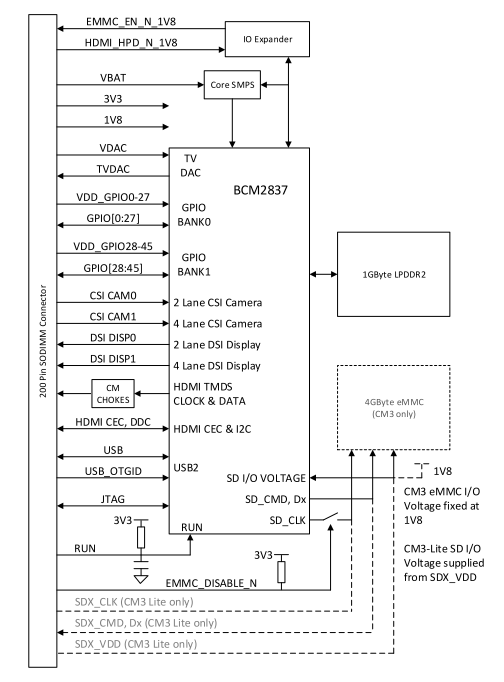
\includegraphics[width = 0.8\textwidth]	{resources/raspsheet}
    	\legend{Fonte:\citeonline{RaspberryPi2016DATASHEETCM3L} }
\end{figure}

Um bom exemplo de um sistema construído utilizando um \textit{Single Board Computer}, é o sistema proposto por \citeonline{jain2014raspberry}, que utiliza Raspberry Pi para automação residencial através da internet utilizando e-mail. 


% =========================================================
\subsection{Internet das Coisas(IoT - Internet of Things)}
% =========================================================

A Internet das Coisas (IoT - \textit{Internet of Things}) é paradigma que está ganhando espaço no cenário moderno de telecomunicações sem fio. Sendo seu conceito básico conectar uma vasta quantidade de coisas ou objetos (casas, carros, sinais de trânsito e outros), fazendo-os interagir entre si para alcançar um objetivo em comum \cite{atzori2010internet}.


Segundo \cite{xia:2012} a Internet das Coisas é um conceito que interligará todos os dispositivos através de sistemas embarcados, formando uma rede de dados inteligente, ubíqua e distribuída. Os dispositivos podem trazer avanços que irão melhorar a qualidade de vida, facilitando a comunicação entre pessoas e dispositivos.

Todos os dispositivos ao nosso redor estarão conectados a internet, isso resultará numa enorme quantidade de dados que terão de ser processados e apresentados sem falhas de forma eficiente. A computação em nuvem pode oferecer uma infraestrutura de ponta a ponta, entre o dispositivo e o servidor satisfazendo essa demanda de qualquer lugar \cite{Gubbi:2013}.

Internet das Coisas é sobre ampliar o escopo de conexões para objetos que não são convencionais de estarem conectados à rede. Por esse motivo uma grande quantidade de soluções de comunicação foram introduzidas, visando o melhor custo energético \cite{siekkinen2012low}. 
% E a utilização dessa visão neste trabalho será onde 

Na tentativa da caracterização da Internet das Coisas, A \autoref{fig:iotoverview} coloca os principais conceitos, tecnologias e padrões na visão desse paradigma, destacando e classificando as diferentes visões que resultam na Internet das Coisas, mostrando o melhor resultado de uma convergência.

 \begin{figure}[H]
	\centering
    	\caption{\label{fig:iotoverview} Paradigma "Internet das Coisas" (IoT) como resultado da convergência de diferentes visões }
		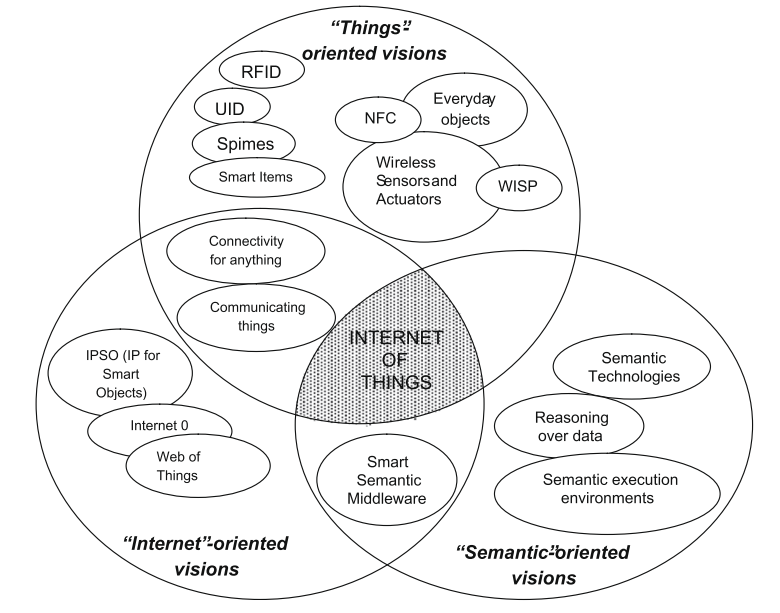
\includegraphics[width = 0.8\textwidth]	{resources/iotoverview}
    	\legend{Fonte: \cite{atzori2010internet}}
\end{figure}

\todo[inline]{Apresentar um exemplo detalhado de IoT}


% =========================================================
\subsection{Baixo consumo de energia}
% =========================================================

Os dispositivos que compõem a Internet das Coisas são caracterizadas por utilizar poucos recursos, em termos de computação e capacidade energética. Isso requer certa atenção, já que novos projetos terão que levar em consideração à eficiência dos recursos e problemas de escalabilidade \cite{atzori2010internet}.

Com o avanço da Internet das Coisas, uma grande demanda de dados surgiu e por sua vez a alocação e gerenciamento de dados se tornaram um problema crítico. Atualmente a internet utiliza 5\% da energia gerada com a solução desses tipos de problemas, e tende a crescer cada vez mais~\cite{Gubbi:2013}.



%Geralmente há restrições no \textit{hardware} e \textit{software}\todo{Apresentar exemplos}. As restrições de \textit{hardware} ajudam a limitar a utilização de recursos energéticos e monetários, e as de \textit{software} limitam o programa a um determinado ciclo, podendo esse ser determinístico ou/e tempo real, reagindo de forma rápida e tolerante a falhas. Essas restrições são dadas pois um sistema embarcado faz parte de um sistema maior, muito mais composto. %informações do slide irei citar 19/01/18

Um sistema embarcado é projetado para executar tarefas específicas, limitando alguns recursos como memória RAM, armazenamento, periféricos e ciclos de processamento e velocidade de processamento. Um exemplo prático é adicionar mais linhas de códigos, usando mais armazenamento, melhorando o tempo de execução do código, outro exemplo é reduzir a velocidade de processamento para reduzir o consumo energético \cite{white:2011}.

De acordo \citeonline{Marwedel:2010}, que descreve uma série de requisitos e abordagens para especificar um dado sistemas embarcados, essas especificações geram modelos do sistema em desenvolvimento. Esses modelos são descritos em linguagens, essas linguagens devem ser capaz de representar alguns características, bem como:
\begin{itemize}
    \item \textbf{Sincronização e Comunicação}: onde os componentes devem se comunicar e estarem sincronizados. sem comunicação não há cooperação entre eles.
    
    \item \textbf{Comportamento Temporal}: levando em consideração há existência de muitos sistemas embarcados em tempo real. Sendo uma das características mais importantes de alguns sistemas embarcados. Na ciência da computação o tempo é dado de maneira abstrata, a notação $O$ é um desses exemplos, que reflete o grau de crescimento de uma função, usado frequentemente para medir o tempo de execução de algoritmos, mas falha ao descrever a execução real de tempo.
    Para sistemas em tempo real, é necessário quantificar o tempo. Para isso algumas técnicas podem ser utilizadas, como: \textbf{medir o tempo utilizado}, meios de \textbf{atrasar um processo} por determinado período de tempo, \textbf{especificar \textit{timeouts}}.  
    
    \item \textbf{Propriedades não-funcionais}: Sistemas embarcados em desenvolvimento devem possuir um número de propriedades não-funcionais, como tolerância a falha, tamanho, extensibilidade, perspectiva de vida, consumo energético, peso e outros.
\end{itemize}

\citeonline{Marwedel:2010} ainda afirma que melhorar as tecnologias de baterias nos ajudará a consumir mais energia, mas o limitação térmica nos impede de utilizar essa energia por muito tempo, devido a problemas de superaquecimento do dispositivo. Devido a esses problemas de temperatura, dispositivos estão sendo projetado com sensores para detectar quando há superaquecimento, regulando o dispositivo para o evitar que isso aconteça. 


% =========================================================
\section{Modelos formais para verificação de sistemas}
% =========================================================
%falar sobre verificação de sistemas. A importância e onde é usada. Falar sobre modelos formais. Falando que a seção fala sobre exemplos de modelos formais. 
 
De acordo com \citeonline{Baier:2008} sistemas de Tecnologia da Informação e Comunicação (TIC) estão crescendo rapidamente, e seu funcionamento de forma eficaz é fundamental. Esses sistemas estão se tornando cada vez mais complexos e estão ganhando espaço no cotidiano através da internet e de todos os tipos de sistemas embarcados. Sistemas TIC estão por toda parte, eles controlam a maioria dos dispositivos de uso cotidiano\todo{Apresenatar exemplos}.

A dependência do uso de sistemas embarcados tornam sua eficácia fundamental para sociedade. Esses sistemas oferecem um bom desempenho em tempo de resposta e capacidade de processamento. O mal funcionamento desses sistemas podem ameaçar nossas vidas, e podem ter consequências financeiras substanciais para o fabricante. Sistemas TIC eficazes são fundamentais para a sobrevivência de uma empresa.

\todo[inline]{Apresentar exemplo de um falha de SE com resultado critico}

O crescimento na complexidade dos sistemas TIC mostram que eles não estão mais isolados, agora podem fazem parte de um grande sistema, conectando e interagindo com vários outros outros componentes, tornando esses sistemas vulneráveis a erros. 
A concorrência e o não determinismo que são fundamentais para a modelagem dos sistemas integrados, tornando a utilização de técnicas padrões muito difícil.

Técnicas de verificação são aplicadas a sistemas TIC de forma mais confiável. A verificação de sistemas trabalha pra estabelecer que o produto possua certas propriedades, como certificar que o sistema não entre em uma situação de \textit{deadlock}. A falha é encontrada quando o sistema não cumpre todas as propriedades especificadas\todo{Adicionar referência}.


%\subsection{Máquina finita de Estados}
%yMáquina finita de estados é um automato que ajuda a demonstrar o fluxo de um sistema computacional. (pré-texto) 

% =========================================================
\subsection{UML}
% =========================================================

Segundo \citeonline{rumbaugh2017unified} UML (\textit{Unified Modeling Language)} é uma linguagem de modelagem visual que tem como intuito de utilizar todos os métodos de desenvolvimento de software, extraindo melhor para especificar, visualizar, desenvolver e documentar os artefatos de um sistema em nível de software, capturando estáticas informais e dinâmicas do comportamento de um sistema.

\todo[inline]{Descrever os tipos de diagramas das UML e o objetivo de cada um deles.}

A utilização de UML nesse trabalho se dará pela utilização de diagramas de sequência que mostrarão como o fluxo do software irã ocorrer. De acordo com \citeonline{rumbaugh2017unified}, diagramas de sequência mostram a iteração em uma forma bidimensional, onde o eixo vertical é o tempo de vida do processo e o eixo horizontal mostra as regras de transição como pode ser visto na Figura~\ref{fig:sequencerumbaugh}. %Essas regras são definidas pelas setas que são os processos do software.

\todo[inline]{Explicar a Figura~\ref{fig:sequencerumbaugh}}

Já \citeonline{Cunha2011FormalContext} diz que diagramas de sequência as ações são organizadas por tempo\todo{Corrigir esta frase}, mas não exploram as relação dos objetos. Os diagramas de sequência mostram todo o processo de trocas de mensagens dos objetos, mapeando todo o ambiente mostrando como os objetos colaboram entre si para obter sucesso. Um exemplo é a \autoref{fig:sequencerumbaugh}, que mostra um diagrama de sequencia, com ator, processos e ações que são executas em certa ordem. 
 \begin{figure}[H]
	\centering
    	\caption{\label{fig:sequencerumbaugh} Diagrama de sequência }
		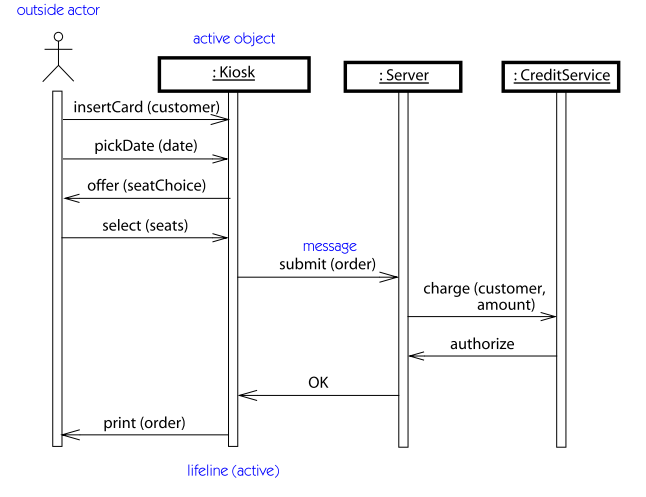
\includegraphics[width = 0.8\textwidth]	{resources/sequencediagramrumbaugh}
    	\legend{Fonte: \cite{rumbaugh2017unified}}
\end{figure}




%falar o que é. pra que é usado, e onde será usado no trabalho

% \todo{Computer vision is a vast fi eld. Th is book will give you a basic grounding in the fi eld, but we also recom- mend texts by Trucco [Trucco98] for a simple introduction, Forsyth [Forsyth03] as a comprehensive refer- ence, and Hartley [Hartley06] and Faugeras [Faugeras93] for how 3D vision really works}
% wa

\subsection{Redes de Petri}

Redes de Petri são modelos gráficos e matemáticos que podem ser aplicados em diversos sistemasa\todo{Exemplos}. Um método capaz de descrever e analisar as transições do sistema, podendo ele ser concorrente, assíncrono, distribuído, paralelo e não-determinístico. O modelo gráfico é capaz de auxiliar na visualização do fluxo, e a ferramenta matemática pode estruturar equações matemáticas para validação de propriedades formais do sistema analisado. O comportamento de sistemas pode ser descrito em estados, um estado em uma rede de Petri é alterado de acordo com a regra de transição~\cite{murata:1989}.

\todo[inline]{Apresentar a definição formal de uma RP.}

Segundo \citeonline{rumbaugh2017unified}, ainda que uma máquina de estados seja bem estruturada, um grupo de transições pode levar a sérias inconsistências, incluindo \textit{deadlocks} e outros problemas. Esses problemas foram bastante estudados na teoria das redes de Petri. 

 \begin{figure}[H]
	\centering
    	\caption{\label{fig:petri}Regra de transição}
		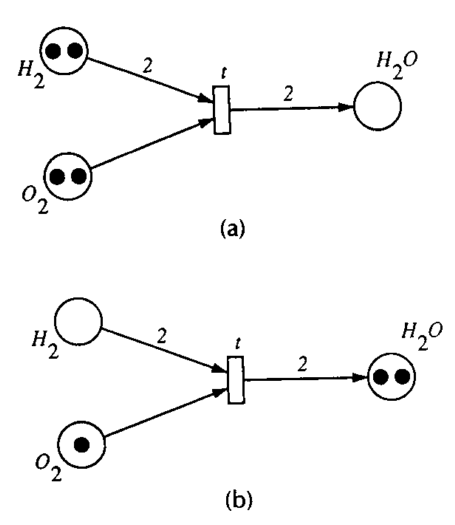
\includegraphics[width = 0.3\textwidth]	{resources/petri}
    	\legend{Regra de transição, (a) aceitação antes da transição \textbf{\textit{t}}. (b) iteração após aceitação de \textbf{\textit{t}}, \textbf{\textit{t}} está desativado.\cite{murata:1989}}
\end{figure}

\todo[inline]{Seção muito raza, explicar as propriedades de RP com exemplos, e então apresentar um exemplo prático tipo um semaforo.}

\section{Visão Computacional}

A visão humana não tem dificuldades em identificar pequenas variações na translucidez e sombreamento em imagens, distinguindo os objetos da imagem que é fundo. Temos certa facilidade em identificar estruturas tridimensionais, podemos diferenciar formatos, texturas, cores e pessoas em imagens, e até mesmo dizer que sentimentos eles podem estar sentindo, apenas olhando fotos \cite{szeliski2010computer}.
% 
A visão computacional é uma forma de emular a visão humana, possuindo imagens como entrada, e sua saída é a interpretação dessa imagem \cite{marengoni:2009}.

\citeonline{bradski:2008} definem uma parte da vasta área da visão computacional como uma transformação de dados de uma imagem em uma nova representação para atingir um objetivo específico, como deixar a imagem em escala de cinza. Essas transformações precisam de contexto, como especificar distância, referências de onde a imagem foi tirada, ou o que pode conter na imagem.

\begin{figure}[h]
	\caption{\label{fig:grayscaleex}Aplicação de uma equalização de histograma, em nível de cinza, onde a placa do veículo pode ser lida (direita).}
	\begin{center}
	    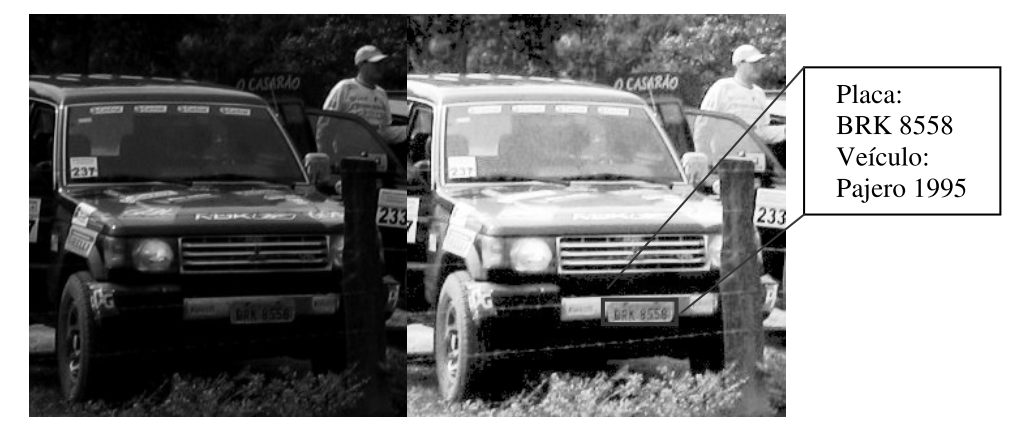
\includegraphics[width=.7\textwidth]{resources/grayscaleex}
	\end{center}
	\legend{Fonte: \cite{bradski:2008}}
\end{figure}


De acordo com \citeonline{marengoni:2009}, o processamento da imagem geralmente é a primeira etapa do processo de visão computacional, podendo ser dividido em três níveis: 
% baixo-nível, nível-médio e alto-nível.

\todo[inline]{Figuras não mencionadas no texto, corrigir}

\todo[inline]{Explicar o resultado das figuras em cada item}

\begin{itemize}
\item Baixo-nível: 
	Pode ser associado a operações como redução de ruídos ou níveis de contraste da imagem. 
   \begin{figure}[h]
	\caption{\label{fig:blur}Aplicação de filtro Gaussiano para remoção de ruídos}
	\begin{center}
	    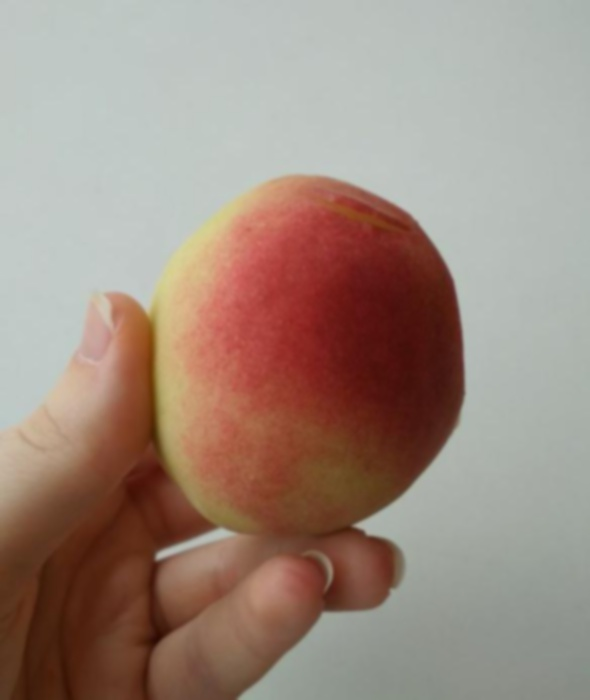
\includegraphics[width=0.3\textwidth]{peachs/blur}
	\end{center}
	\legend{Fonte Própria}
\end{figure} 
\item Nível-médio:
	São operações associadas a operações de segmentação de imagem ou reconhecimento de objetos na imagem.   
       \begin{figure}[H]
	\caption{\label{fig:segment}Segmentação com base nas cores da imagem com sobreposição para identificação de pêssegos.}
	\begin{center}
	    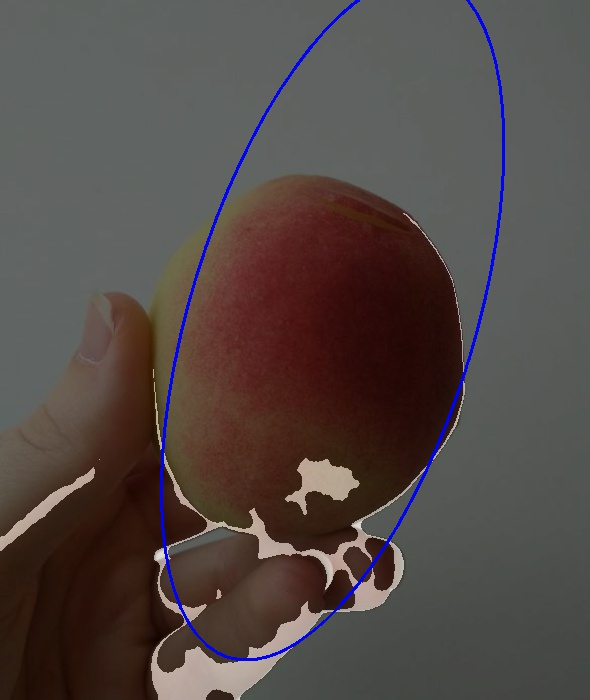
\includegraphics[width=0.3\textwidth]{peachs/identified}
	\end{center}
	\legend{Fonte Própria}
\end{figure}

\item Alto-nível:
São relacionados a tarefas de cognição associadas com a visão humana.
       \begin{figure}[h]
	\caption{\label{fig:machineflow}Identificação de objetos utilizando aprendizado de máquina.}
	\begin{center}
	    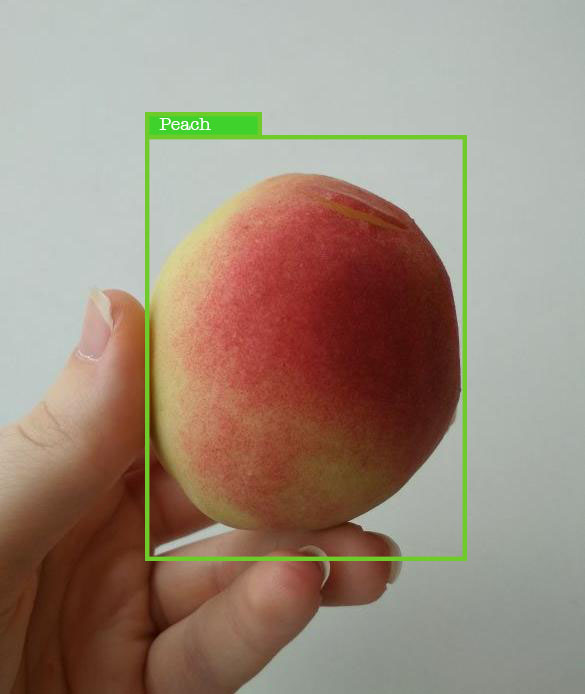
\includegraphics[width=0.3\textwidth]{peachs/tensorflow}
	\end{center}
	\legend{Fonte Própria}
\end{figure}
	
\end{itemize} 


\todo[inline]{Apresentar as outras etapas do processo de visão computacional}


% ----------------------------------------------
% ---------------------------------------------- 
\subsection{Representação de Imagens Digitais}
Uma imagem pode ser definida como uma função bidimensional, $f(x,y)$, onde $x$ e $y$ são coordenadas espaciais, e a amplitude de $f$ em qualquer par de coordenadas $(x,y)$ é chamada de intensidade da imagem, naquele determinado ponto. Quando $x,y$ e os valores de amplitude de $f$ são finitos, chamamos a imagem de imagem digital. Uma imagem digital é composta por um número finitos de elementos, cada um tendo seu próprio ponto e posição específicos. Esses elementos se referem à elementos de imagem, \textit{pels} e \textit{pixels} \cite{gonzalez1992digital}. 

O termo processamento de imagens digitais normalmente se referem ao processamento de imagens bidimensionais por computadores. Uma imagem digital é um vetor de números reais ou números complexos representados por uma quantidade finita de \textit{bits}.
Na representação de imagem devemos nos preocupar com a caracterização e quantidade de elementos que representam a imagem (\textit{pixels} ou \textit{pels}). Em geral qualquer função bidimensional que contém alguma informação pode ser considerada uma imagem. O principal requisito para o processamento de imagens digitais é que ela seja amostrada e logo em seguida quantificada. A taxa de amostragem, que são os \textit{pixels} por unidade de área, tem de ser grande o suficiente para preservar uma quantidade de informações úteis na imagem. A quantização da imagem é a conversão analógica para digital de uma imagem amostrada para um número finito de níveis de cinza \cite{jain1989fundamentals}.
 \begin{figure}[h]
	\caption{\label{fig:digitalproc}Típica sequência de processamento de imagem digital.}
	\begin{center}
	    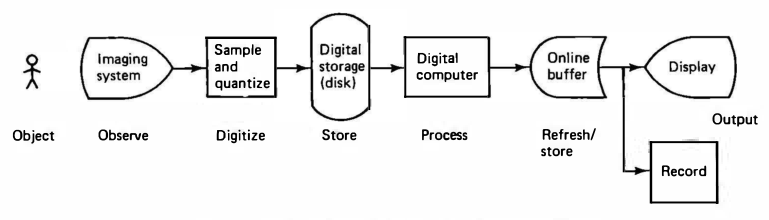
\includegraphics[width=.9\textwidth]{resources/digitalproc}
	\end{center}
	\legend{Fonte: \cite{jain1989fundamentals}}
\end{figure}

\todo[inline]{Descrever a representação com exemplos práticos}

%\subsection{Pré-processamento de Imagem}

%\subsection{Segmentação e Detecção de Objetos}

%\subsection{Pós-Processamento}

\section{\textit{Frameworks} para identificação de imagem}

Nesta sessão iremos abordar \textit{frameworks} para identificação e classificação de imagens, onde são usando, as vantagens e desvantagens em  relação a métodos convencionais e tecnologias que utilizam \textit{frameworks} para suas atividades. %melhorar depois%

% \todo{falar sobre aprendizado de máquina na sua utilização no projeto: como caixa preta}
%De acordo com \cite{papag} As dificuldades na identificação de objetos de interesse do mundo real, como rostos e pessoas são dadas pela complexidade desses tipos de objetos, uma quantidade significante de variedade de cores e texturas e o contraste com o fundo da imagem. Em comparação com a classificação de padrões, onde é necessário decidir entre classes bem definidas, na detecção de objetos é necessário diferenciar a classe de objeto para o que é o resto. 

\todo[inline]{Criar uma seção Aprendizagem de Máquina}

\subsection{\textit{Tensorflow}: Um \textit{Framework} de Código Aberto para Aprendizagem de Máquina}

Tensorflow é um \textit{framework} para operações computacionais, tendo uma grande biblioteca permitindo o desenvolvimento para diferentes plataformas, de \textit{clusters} de servidores até dispositivos móveis. Tensorflow tem grande facilidade de lidar com problemas de aprendizado de máquina e \textit{deep learning}, podendo ser usado em diversos domínios científicos \cite{tensorflow2015}. A utilização do \textit{framework} será de extrema importância nas classificações de imagens que serão processadas.

\todo[inline]{Ampliar a descrição e adição de exemplos}

\subsection{YOLO: Detecção de Objetos em Tempo Real}
\todo{fazer a mesma coisa pro YOLO (mesma coisa do tensorflow)}

\todo[inline]{Ampliar a descrição e adição de exemplos}

%\section{Aprendizagem de máquina}
%Falar o que é. onde é usado, mostrar exemplos (muitas imagens), visão geral pra ter uma ideia do que é capaz

%\subsection{Redes Neurais}
%\todo{num sei}

%\subsection{Redes Neurais Convolutivas}
%\todo{num sei}

%\section{Reconhecimento de Padrões}


%\subsection{Aprendizado de máquina} 


%\subsection{Classificação de Padrões}


 
% \subsubsection{Homomorphic filtering} 
% 	O filtro homomórfico (\textit{homomorphic filter}) é um filtro de frequência usado para corrigir iluminações não uniformes e realçar o contraste na imagem processada \cite{bazeille2006}.
     
%  \begin{figure}[H]
% 	\centering
%     	\caption{\label{fig:homofilter}Homomorphic Filtering}
% 		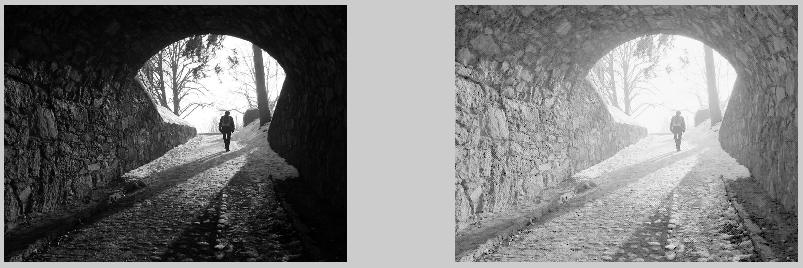
\includegraphics[width = 0.9\textwidth]	{resources/homofilter}
%     	\legend{\textit{Homomorphic filtering}, usando \textit{Butterworth High Pass Filter} para fazer a filtragem \cite{mathworks:2008}}.
% \end{figure}

%     %Considerando o modelo de reflectância, assumimos que uma imagem é o produto descrito pela equação:
%     \[
%     %	f (x,y) = i(x,y).r(x,y)
%     \]
%     %Sendo $f(x,y)$ é a imagem captada por um sensor ótico, $i(x,y)$ o fator multiplicativo de iluminação e $r(x,y)$ a função de reflectância. 
    

% \subsubsection{Anisotropic filtering}
% O Filtro anisotrópico permite a simplificação de atributos da imagem para melhorar a segmentação,  suavizando as partes homogêneas preservando as bordas e melhorando-as.

%  \begin{figure}[H]
% 	\centering
%     	\caption{\label{fig:anisifilter}Anisotropic Filtering}
% 		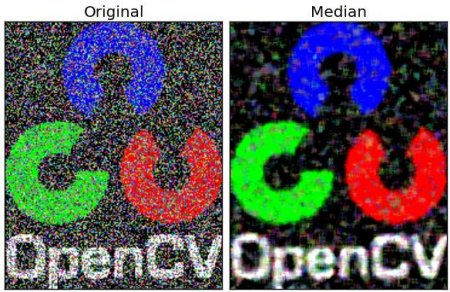
\includegraphics[width = 0.6\textwidth]	{resources/anisifilter}
%     	\legend{Fonte:\cite{mathworks:2008}}.
% % \end{figure}

% \subsection{Sensores de Aquisição de Imagens}
% Segundo \citeonline{Lu:2017}, o som pode ser usado para mapear ambientes, emitindo um pulso que reflete no fundo do oceano criando um sonograma. As imagens obtidas por este sonar se assemelham a imagens óticas, com níveis de detalhes bem superiores. O reflexo criado por esse sonar tem formato de leque, com a medida que o pulso se movimenta, os reflexos irão criar séries de linhas de imagem, perpendiculares ao feixe.  

% \subsection{Ferramentas para reconhecimento de images}
% \todo{Definir junto ao método proposto}


    


% ----------------------------------------------------------
% Revisão de Literatura
% ----------------------------------------------------------
\chapter{TRABALHOS CORRELATOS}
\label{chapter:correlatos}

Neste capítulo serão apresentados e discutidos os principais trabalhos existentes na literatura que se relacionam com os tópicos que formam a base para o desenvolvimento deste trabalho, com ênfase em: Pré-processamento de Imagem, Segmentação e Detecção de Objetos, Pós-processamento e Reconhecimento de Padrões.


% OS TEXTOS ABAIXO DEVEM IR PARA CONCLUSÃO PARCIAIS
% O projeto proposto visa o desenvolvimento de um sistema embarcado, conectado a uma central para processamento de imagem através de uma rede sem fio. O projeto encontra-se em desenvolvimento, já tendo realizado diversas atividades tais como: revisão da literatura; diagramação das etapas do método proposto; e elaboração de um método para identificação e classificação de imagens. 

  
% Visando documentar o fluxo de execução do método proposto neste trabalho, foi realizado a diagramação do método proposto, utilizando diagramas da UML e caixas, com a especificação de tecnologias como linguagens de programação e métodos encontrados na literatura a serem utilizadas no projeto do sistema computacional proposto neste trabalho. Logo, o sistema proposto é apresentado como um sistema embarcado usando  microcontroladores (neste caso, neste projeto esta sendo testado as plataformas Arduino e Raspberry Pi), sensores óticos, etc. 

% O sistema embarcado proposto será baseado em detecção via um sensor de captura ótica, que ficará submerso em água, acoplados à uma boia, que terá um conexão sem fio com um celular ou computador. O pré-processamento da imagem é feito com diversos filtros e processos para correção de anomalias na imagem.


% O módulo  de detecção de objetos do sistema proposto, ainda em desenvolvimento, está sendo aperfeiçoado para interagir de forma inteligente com o ambiente observado, isso significa que filtros serão automaticamente aplicados para melhorar a detecção de objetos em ambiente com pouca iluminação e com alta turbidez. Com base na estrutura do sistema computacional proposto, ainda identificamos alguns desafios a serem superados para a conclusão do trabalho proposto, tais como: a integração dos diferentes módulos (exemplo, detecção de objetos) em um único sistema; consumo  energético; estrutura e prototipação dos sistema em ambientes reais como rios. 
	

 

%\section{Análise e publicação de resultados}
%A Tabela detalha os resultados gerais de publicações identificadas pela máquina de busca, bem como o número de publicações aceitas em cada um dos filtros executados, de acordo com a expressão de busca executada na biblioteca Scopus. \textcolor{red}{adicionar tabela de resultados.}


% \section{Análise dos trabalhos correlatos}
% Nesta seção serão serão feitas análises dos trabalhos correlatos, mostrando as diferenças entre o projeto proposto e os trabalhos encontrados, como tecnologias e estruturas utilizads.

% ================================================
\section{DeepFish: Accurate underwater live fish recognition with deep architecture}
% ================================================

Um \textit{framework} baseado em uma rede neural convolutiva foi proposto por \citeonline{Qin:2016} para reconhecimento de peixes em vídeos gravados submersos em águas oceânicas. No trabalho as imagens de fundo são removidas utilizando métodos baseados em decomposição de matrizes esparsas e de baixo nível, removendo assim apenas o fundo da imagem, deixando somente o peixe.

Os dados extraídos são passados para camadas de convolução depois para uma camada não linear, em seguida é feita a classificação utilizando SVM (Support Vector Machine)\cite{cortes1995support}. A taxa de aprendizado diminui a medida que a quantidade de parâmetros são adicionados, necessitando assim de uma otimização no filtro de aprendizado. 

O método do trabalho de \citeonline{Qin:2016}, pode ser visto na \autoref{fig:trainignqin}, onde os passos do \textit{framework} são mostrados. Onde os filtros são escolhidos, as imagens processadas pela rede neural profunda e processos para extração de atributos, após essas etapas a saída final alimenta uma máquina de vetor de suporte linear.
\begin{figure}[h]
	\caption{\label{fig:trainignqin}\textit{Pipeline} do \textit{framework} proposto.}
	\begin{center}
	    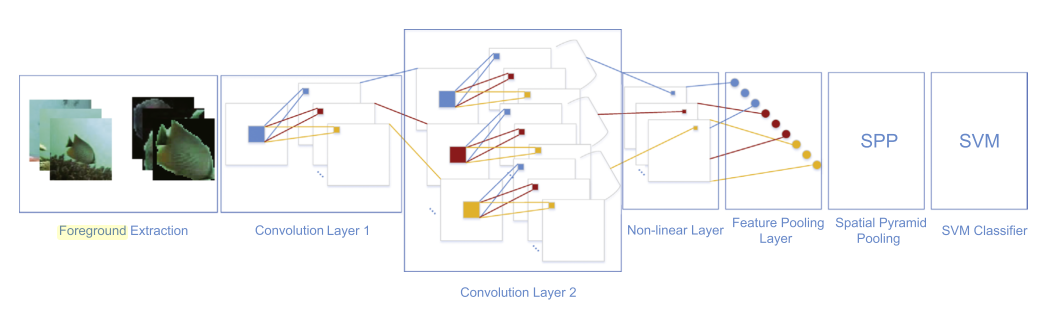
\includegraphics[width=1\textwidth]{resources/trainingqin}
	\end{center}
	\legend{Fonte: \cite{Qin:2016}}
\end{figure}
   

Similar ao trabalho de \citeonline{Qin:2016}, o método apresentado nesse trabalho de conclusão de curso propõe um método para detecção
% , porém não à identificação 
de imagens, onde a classificação será feita utilizando métodos baseados em \textit{Convolutional Neural Network} assim como no trabalho de \citeonline{Qin:2016}.

%Com o \textit{framework} proposto pelo trabalho espera-se avanços na área de pesquisas sobre reconhecimento de peixes, explorar soluções no reconhecimento de objetos submersos. Beneficiar biológos, ecologistas e fins comerciais como fazendas de peixes.

% ================================================
\section{A Feature Learning and Object Recognition Framework for Underwater Fish Images}
% ================================================

\citeonline{Chuang2016AImages} propõe um \textit{framework} para reconhecimento de peixes em baixo d'água, que consiste em uma técnica de aprendizagem totalmente não supervisionada e um classificador resistente a erros, conforme \autoref{fig:trainingchuan}. Os dados são iniciados com base em algumas características (como formato do contorno do peixe), depois passados por alguns critérios de classificação com base nessas características. 

A \autoref{fig:trainingchuan} ilustra o classificador, que tem uma abordagem não supervisionada que gera uma classe de hierarquia binária, onde cada nó é um classificador. Os experimentos mostram que o \textit{framework} proposto é preciso tanto em situações onde a base de dados é pública quanto em ambientes controlados com alta incerteza.

\begin{figure}[h]
	\caption{\label{fig:trainingchuan}Proposta de treinamento não supervisionada.}
	\begin{center}
	    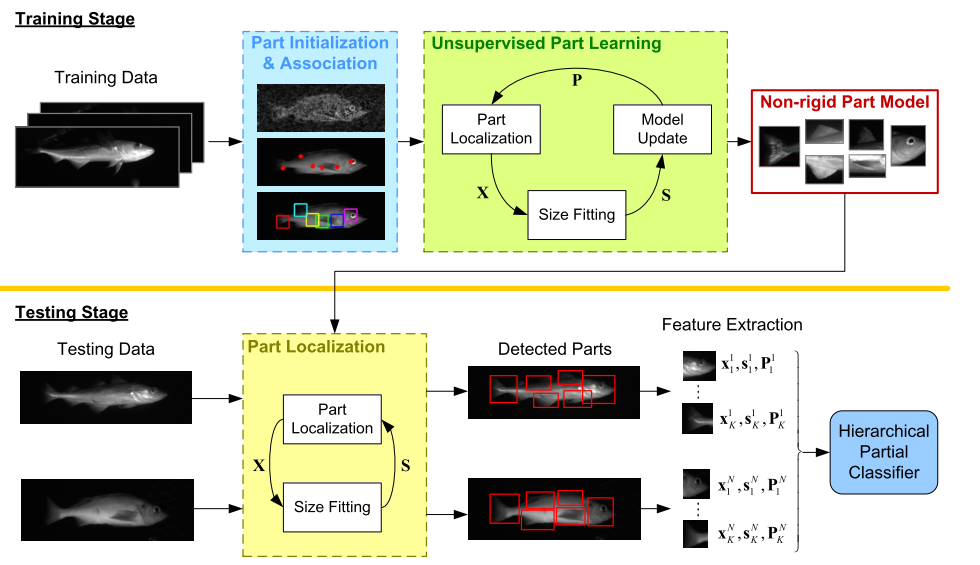
\includegraphics[width=0.9\textwidth]{resources/training}
	\end{center}
	\legend{Fonte: \cite{Chuang2016AImages}}
\end{figure}

A utilização do trabalho de \citeonline{Chuang2016AImages} como referência irá auxilar em uma abordagem de aprendizado resistente a erros, que irá auxiliar na confiabilidade de informação, uma vez que o sistema proposto neste trabalho irá auxilar mergulhadores em lugares de riscos, em águas com alta turbidez. 

% ================================================
\section{A Vision Based System for Object Detection in Underwater Images.}
% ================================================

O trabalho de \citeonline{FORESTI2000AImages} propõe um sistema (veículo autônomo) para detecção e rastreio de objetos submersos em água, conforme fluxograma na ~\autoref{fig:forestflow}, o sistema faz detecção automática de canos (que podem se estender por quilômetros) e posicionamento autônomo baseado nas detecções.

No método proposto por \citeonline{FORESTI2000AImages} são aplicados alguns filtros para compensação de cor e dimensionamento na imagem. Depois do dimensionamento essas imagens ganham tamanhos de $1/16$ para detecção de bordas (para encontrar canos) e $1/32$ para encontrar anodos em canos.
\begin{figure}[h]
	\caption{\label{fig:forestflow}Proposta do sistema.}
	\begin{center}
	    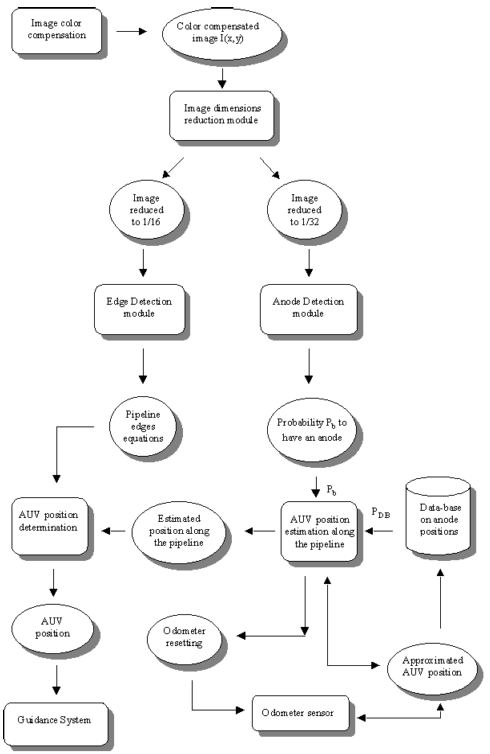
\includegraphics[width=0.5\textwidth]{resources/flowchartforest}
	\end{center}
	\legend{Fonte: \cite{FORESTI2000AImages}}
\end{figure}

A identificação dos objetos é feita utilizando redes neurais, que classificando a imagem em tempo real, verificando se há obstáculos. Essas informações auxiliam na navegação automática do veículo, traçando rotas e caminhos através das imagens processadas e ressonância geométrica.

O sistema proposto por \citeonline{Gentili2000A.} consegue detectar canos e outras estruturas, mesmo com os problemas causados pela falta de luminosidade, dispersão e atenuação da luz e problemas como areia e detritos sobre canos.

% Comparado ao trabalho que está sendo desenvolvido, um sistema irá trabalhar na detecção de objetos, e estipulação do tamanho desses objetos, afim de avisar os possíveis perigos que se escondem de baixo d'água.

% ================================================
%\section{Automatic Plankton Image Recognition}
% ================================================

%O trabalho de \citeonline{tang1998automatic} propõe um sistema que utiliza redes neurais para classificação de padrões para identificar um grande número de imagens de plânctons, detectadas em tempo real por um sistema de microscópio de vídeo subaquático rebocado. O sistema que utiliza características granulométricas em escala de cinza como um poderoso descritor de padrão que captura as assinaturas de forma e textura, capaz de detectar automaticamente plânctons, auxiliando no rastreio da proliferação da vida marinha que se alimentam de plânctons e entender o complexo ecossistema marinho.

% \begin{figure}[h]
% 	\caption{\label{fig:tangnet} Quantização vetorial de aprendizado da rede neural.}
% 	\begin{center}
% 	    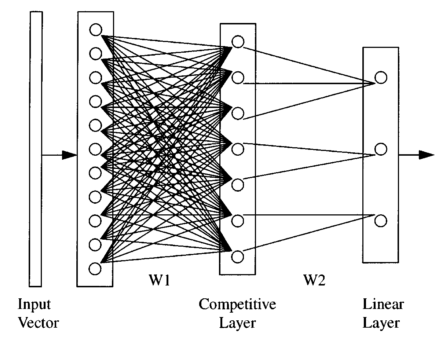
\includegraphics[width=0.5\textwidth]{resources/neuralnet}
% 	\end{center}
% 	\legend{Fonte: \cite{tang1998automatic}}
% \end{figure}

% No trabalho \citeonline{tang1998automatic} o sistema proposto é capaz de identificar plânctons para compreensão de como o ecossistema marinho funciona. Em comparação, o método apresentado neste trabalho de conclusão de curso é proposto um método para detecção, porém não à identificação de objetos em ambiente aquático submersos em águas turvas, mas sim uma classificação de que tipo de objeto e uma especulação do seu tamanho. A classificação será feita utilizando métodos baseados em \textit{Convolutional Neural Network}, utilizando o \textit{framework} \textbf{Tensorflow}.

% ================================================
\section{Automatic underwater image pre-processing}
% ================================================

\citeonline{bazeille2006} propõe um algoritmo para processamento e restauração de imagens de ambiente submersos.  Imagens de ambiente submersos sofrem pela perda de distância na captura, distorção de luz, baixo contraste, baixa saturação de cor e outros problemas. Os métodos de processamento de imagens atuais focam em distorção e atenuação causados pela luz e precisam de conhecimento do ambiente que está sendo estudado. O algoritmo proposto pelo trabalho de \citeonline{bazeille2006} é um algoritmo que automatiza o pré-processamento de imagens submersas. O algoritmo proposto no trabalho de \citeonline{bazeille2006} reduz as pertubações nas imagens submersas, e melhorando a qualidade da imagem.


\begin{figure}[h]
	\caption{\label{fig:bazeillemetod}Aplicação do algoritmo proposto por \cite{bazeille2006} passo-a-passo.}
	\begin{center}
	    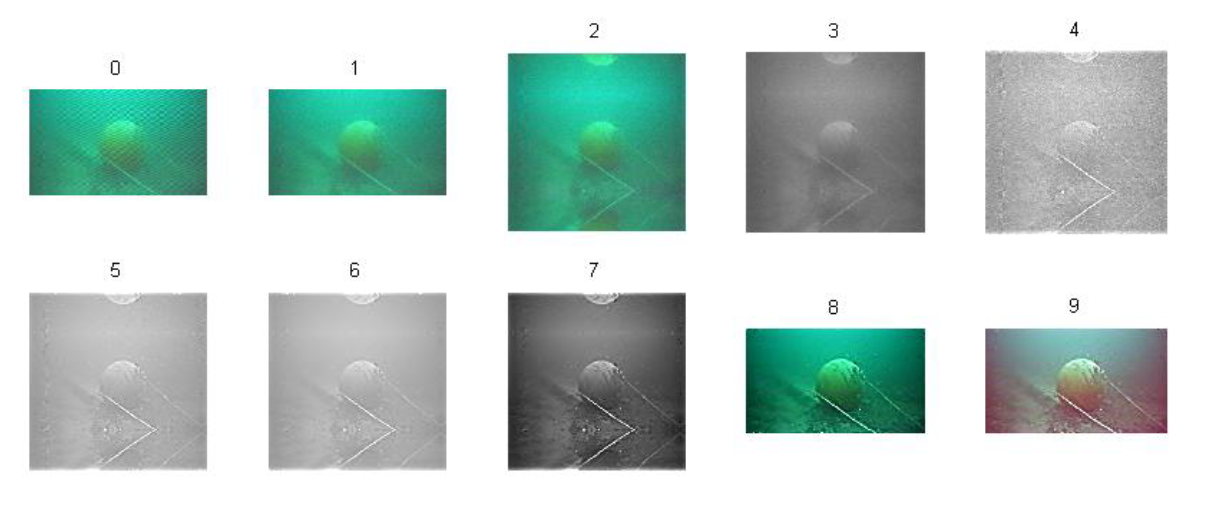
\includegraphics[width=0.9\textwidth]{resources/bazeilemetod}
	\end{center}
	\legend{Fonte: \cite{bazeille2006}}
\end{figure}

A \autoref{fig:bazeillemetod}, mostra o resultado da aplicação de diversas técnicas para processamento de imagem e remoção de pertubações, como atenuações de luz.

O algoritmo proposto por \cite{bazeille2006} utiliza algumas técnicas que serão importantes para o pré-processamento das imagens do sistema computacional proposto nesse trabalho de conclusão de curso, algumas dessas técnicas são:

\begin{description}
    \item[Remoção do padrão \textit{Moiré}]: O padrão Moiré é removido através de uma análise espacial detectando picos nas nas transformadas de \textit{Fourier} e deletando-as assumindo que eles representam padrões Moiré.
    
    \item[Redimensionamento de imagem]: Essa transformação padroniza a imagem facilitando a aplicação de algoritmos como as tranformadas de \textit{Fourier}.
    
    \item[Filtro homomórfico]: Utilizado para correção de iluminação e aprimorar o contraste da imagem.
\end{description}
    

%Processos independentes e sucessivos que corrigem a ilumação não uniforme, supressão de ruídos, melhoria no contraste e ajuste de cor, aplicados com base na detecção de bordas.
%\section{Foreground Extraction of underwater Videos via Sparse and Low-rank Matrix Decomposition}


%\section{Análise dos trabalhos correlatos}
%Nessa sessão será abordado as características similares e comparações dos trabalhos correlatos com o desenvolvimento do trabalho de conclusão de curso. Mostrando as técnicas e métodos utilizados.

%\subsection{Pré-processamento}
%O pré-processamento da imagem é um passo fundamental para poupar processamento, uma vez que será menos dados a serem processados, diminuindo tempo e gastos energéticos, e como o trabalho a ser desenvolvido será um sistema embarcado, o aperfeiçoamento e eficiência são peças fundamentais.

%No trabalho de \citeonline{Qin:2016}, as imagens de fundo são removidas utilizando métodos baseados em decomposição de matrizes esparsas e de baixo nível, removendo assim apenas o fundo da imagem, deixando somente o peixe.

%Já no trabalho de \citeonline{FORESTI2000AImages}, são aplicados alguns filtros para compensação de cor e dimensionamento na imagem. Depois do dimensionamento essas imagens ganham tamanhos de 1/16 para detecção de bordas (para encontrar canos) e 1/32 para encontrar anodos em canos.

%No trabalho de \citeonline{Chuang2016AImages} um filtro Gaussiano é aplicado junto uma transformada de Fourier para estimar a saliência na imagem, em seguida uma máscara é utilizada para descartar pontos no plano de fundo da imagem. em seguida a extração do fundo é feita por técnicas como \textit{GrabCut Segmentation}.

%\begin{itemize}
%\item Reconhecimento de objetos (OR): Algum objeto ou ser vivo foi reconhecido.
%\item Turbidez no ambiente (TA): O ambiente estudado tinha baixa visibilidade e/ou algum tipo de detrito ou interferência .
%\item Sistema desenvolvido para captura de imagens submersas (SC): Algum sistema criado para capturar imagens submersas foi desenvolvido.
%\item Foco em baixo custo (BC): O projeto foi desenvolvido com ideia de baixo custo ou eficiência energética. 
%\end{itemize}


%\begin{table}[H]
%\caption{Comparações}
%\small
%\centering
%\begin{tabular}{|p{8cm}|c | c | c | c |}
 
%	\hline \textbf{Trabalhos} & \textbf{OR} & \textbf{TA} & \textbf{SC} & \textbf{BC}\\ \hline
	
 %   Computer Vision for ocean observing & X & X &  &  \\ \hline
	
  %  DeepFish: Accurate underwater live fish recognition with deep architecture & \centering X & X &  & X \\ \hline
      
  %    A Vision Based System for Object Detection in Underwater Images & X & X & & X  \\ \hline  
      
   %     Automatic underwater image pre-processing &  & X & &   \\ \hline
        
        
    %    A Feature Learning and Object Recognition Framework for Underwater Fish Images &  & X & &   \\ \hline
	%\end{tabular}

%\end{table}




% ----------------------------------------------------------
% Detalhes de Desenvolvimento do Projeto
% ----------------------------------------------------------
\chapter{MÉTODO PROPOSTO}
\label{chapter:metodo}
\section{Visão geral do método proposto}
   
O sistema computacional proposto será estruturado em forma de boia aquática, que será composta com microcontroladores, sensores para análise da água e para a captura ótica, visando adquirir imagens subaquáticas em tempo real. O sistema proposto contará com um módulo de classificação em uma central conectada, onde os dados serão processados e exibidos para o usuário final. 

A interação com a Boia (ainda me desenvolvimento), será através de uma conexão sem fio, como pode ser visto na \autoref{fig:bigpic}, visando mais praticidade para o usuário final, assim como facilidade de transporte da Boia, uma vez que a Boia pode ser energizada utilizando um painel solar.

 
   
%O sistema terá um sensor de captura ótica, que ficará submersos em água, acoplados à uma boia, que terá um conexão sem fio com um celular ou computador.

\begin{figure}[ht]
	\centering
    \caption{\label{fig:bigpic}Visão Geral}
	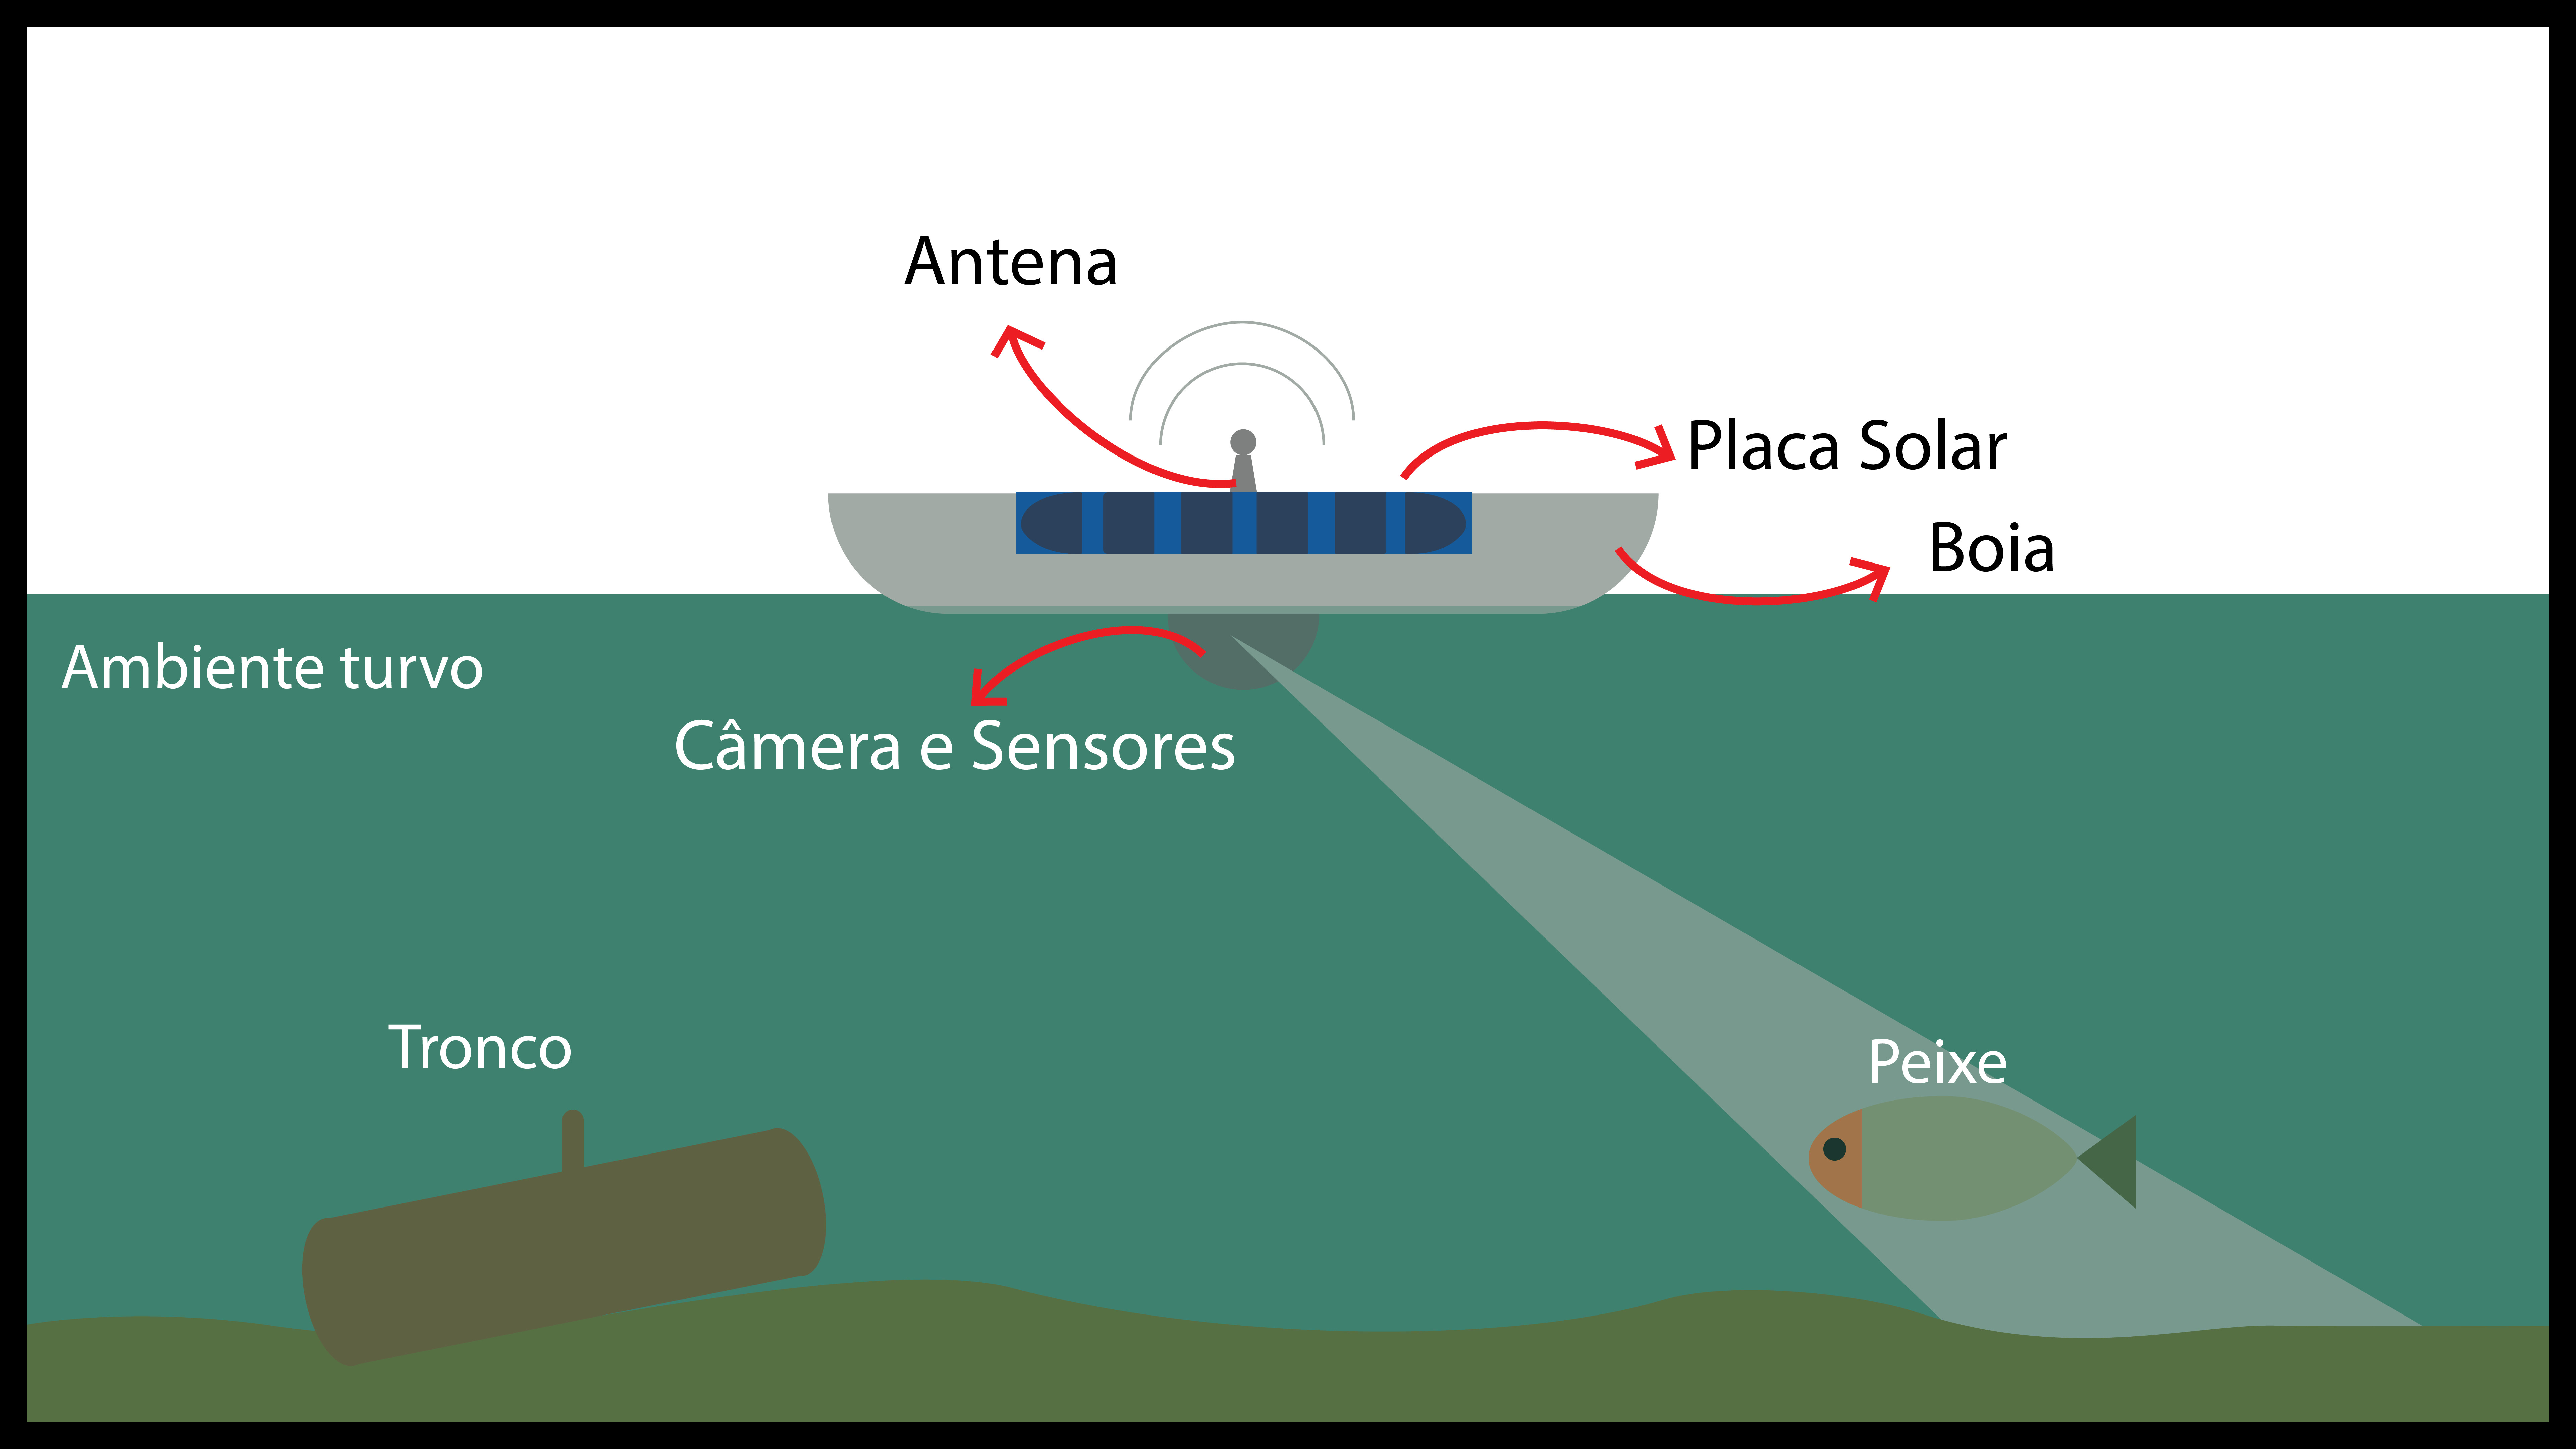
\includegraphics[width = \textwidth]{resources/bugpicturefloater}
    \legend{Fonte Própria}
\end{figure}

Na \autoref{fig:bigpic}, podemos ver como será o funcionamento do sistema computacional proposto em uma situação hipotética, e na \autoref{fig:storyb}, podemos ver como será feita a interação da Boia com a Central, mostrando suas etapas e telas. 

\section{Sistema computacional de suporte a coleta de imagens em ambientes fluviais: Kraken}
%\todo{o que será a boia;
%que sensores irá utilizar;
%como será a conexão com a centra;
%como será a centra;
%falar sobre a possibilidade de adição de sensores;}


A Boia proposta contará com microcontroladores que serão responsáveis por gerenciar os sistemas integrados à mesma, como motores e/ou estabilizadores e sensores para detecção de objetos e captura de imagens dentro do ambiente fluvial com alta turbidez, identificando objetos, classificando-os e especulando seu tamanho. A Boia servirá para facilitar muitas atividades, por exemplo, a prática de mergulho em áreas de risco, onde a visibilidade é quase nula.

A utilização de uma plataforma de sistema integrada (\textit{Single Board Computer}) com uso de microprocessador, contendo várias entradas (digitais e analógicas), irá garantir o suporte para novas extensões como um oxímetro, que irá medir o nível de oxigênio na água. O uso do microprocessador será o meio para interligar a maioria dos sensores e fará a conexão com a central, garantindo que os dados sejam tratados e enviados ao usuário final.


\begin{figure}[ht]
	\centering
    \caption{\label{fig:storyb}\textit{Storyboard}}
	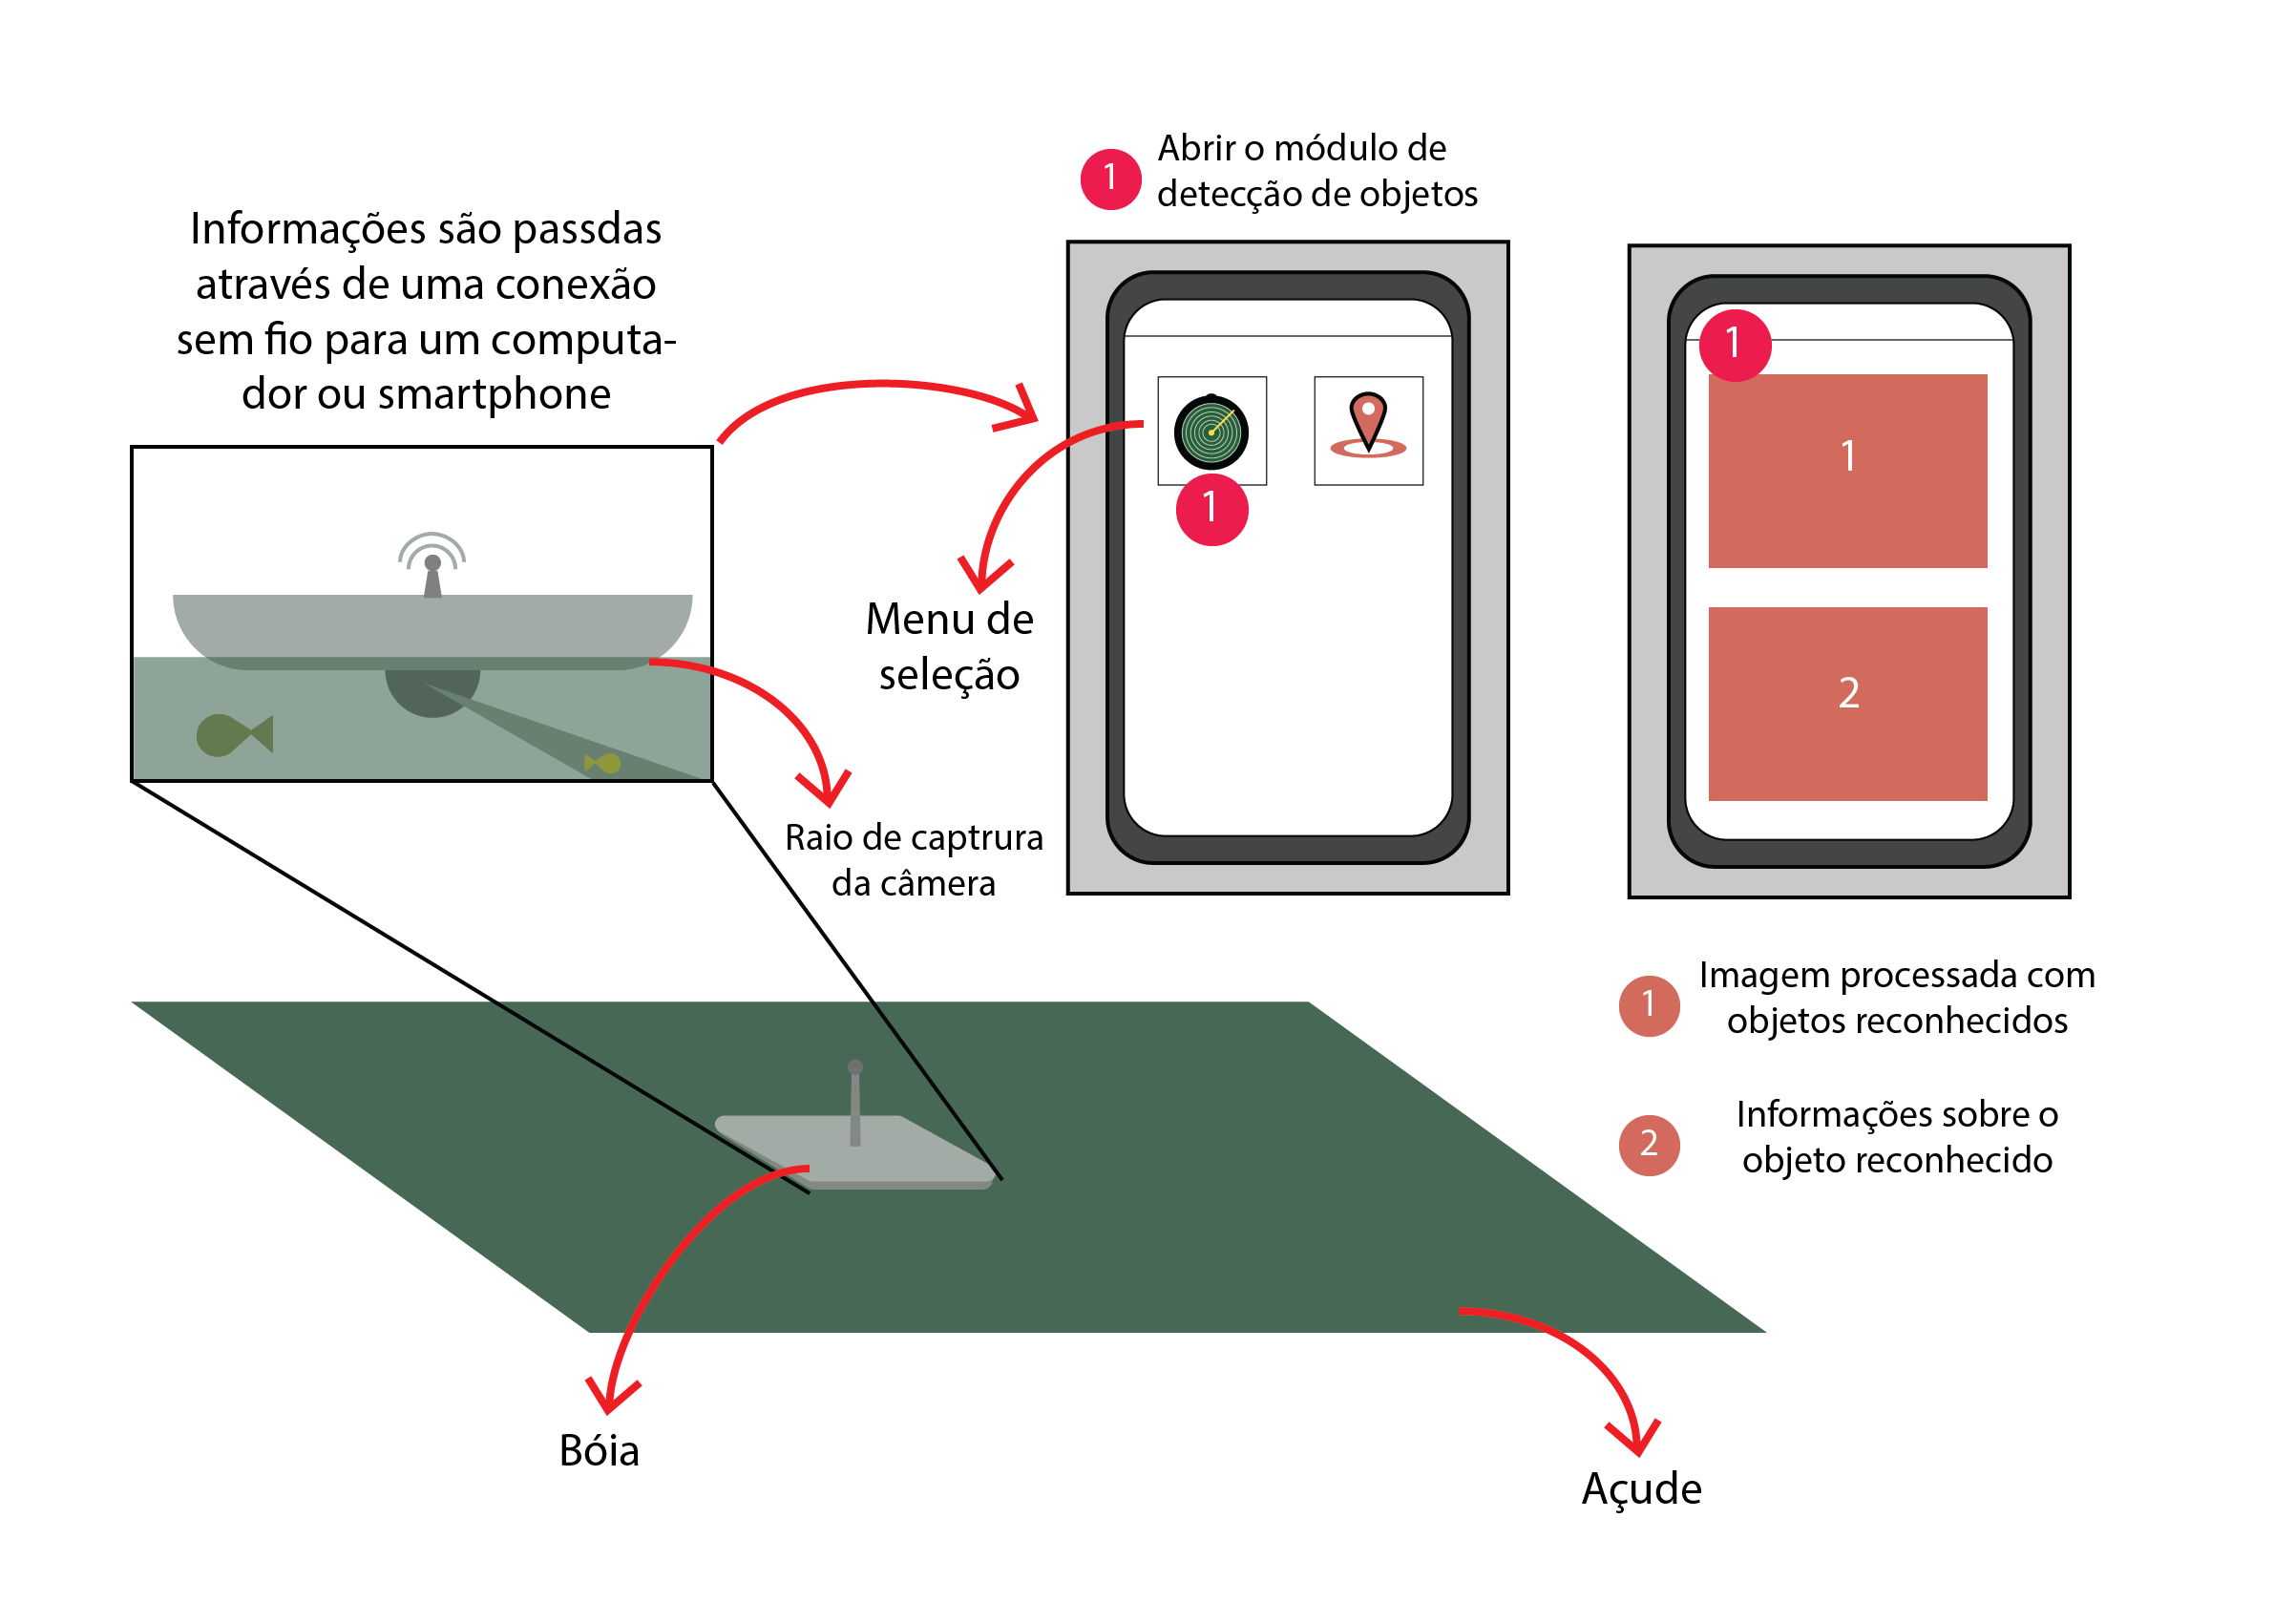
\includegraphics[width = 1 \textwidth]{resources/storyboard.png}
    \legend{Fonte Própria}
\end{figure}

A \autoref{fig:storyb} ilustra como serão as etapas de interação da Boia com a Central, que contará com um aplicativo de auxílio, onde serão exibidos os resultados para o usuário, tais como os dados coletados pela boia, garantindo uma entrega rápida de informação. 

Os dados classificados terão seus tamanhos especulados, e as imagens serão tratadas usando filtros com a biblioteca \textit{OpenCV}\cite{opencv}. A imagem será pré-processada antes de ser enviada ao classificador, isso irá garantir que a imagem esteja em perfeitas condições de classificação.


Além do aplicativo de auxilio, o sistema conta com um modulo de classificação de imagens que pode ser \textit{modelado} de acordo com a necessidade do ambiente, em especifico neste trabalho iremos adotar o \textit{framework Tensorflow}. 



\begin{figure}[ht]
	\caption{\label{fig:fluxcentral}  Fluxo de funcionamento do sistema proposto.}
	 \begin{center}
		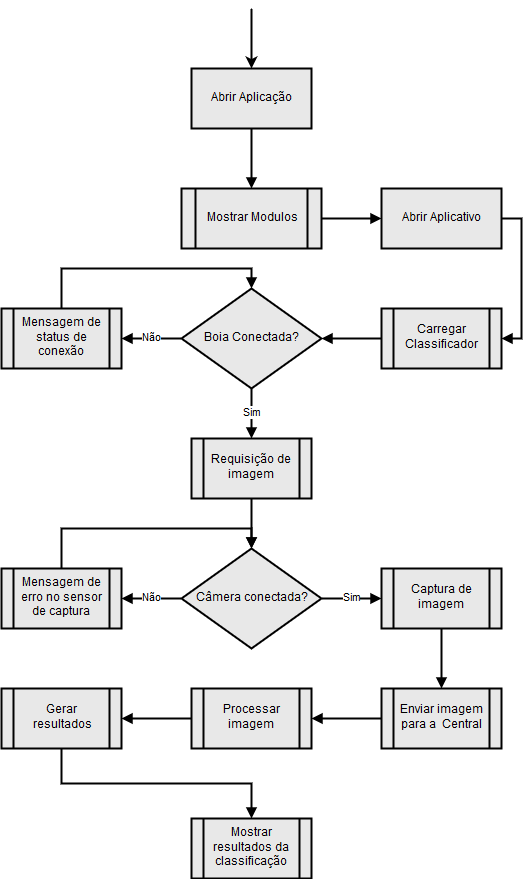
\includegraphics[width = 0.5\textwidth]			{resources/Fluxo-central}
    \end{center}
    \legend{Fonte Própria}
\end{figure}

Como demonstra a \autoref{fig:fluxcentral} o fluxo do sistema com a inicialização da aplicação, onde os módulos serão exibidos, dando opção para usuário abrir a aplicação para classificar e gerar o relatório da imagem. Em seguida a verificação se a Boia está conectada a Central e caso não esteja uma mensagem é retornada informando para o usuário que a conexão falhou, caso contrário, uma requisição de imagem é solicitada à Boia, onde mais uma vez será verificada a conexão com o sensor óptico, enviando mensagem de falha caso esteja desconectado. Uma vez que o a imagem é enviada para a Central, o módulo de classificação irá pré-processar a imagem caso seja necessário, e quando a imagem estiver adequada será processada e um relatório será gerado e exibido para o usuário.

O diagrama de sequência representeado pela \autoref{fig:seqkraken} mostra a sequência de interações do sistema, tais como: a interação do usuário com a Central; e da Central com a Boia. As condições caso haja falha nas conexões com os sensores e como proceder caso essas falhas sejam encontradas.

\begin{figure}[ht]
	\caption{\label{fig:seqkraken}  Diagrama de sequencia do sistema proposto.}
	 \begin{center}
		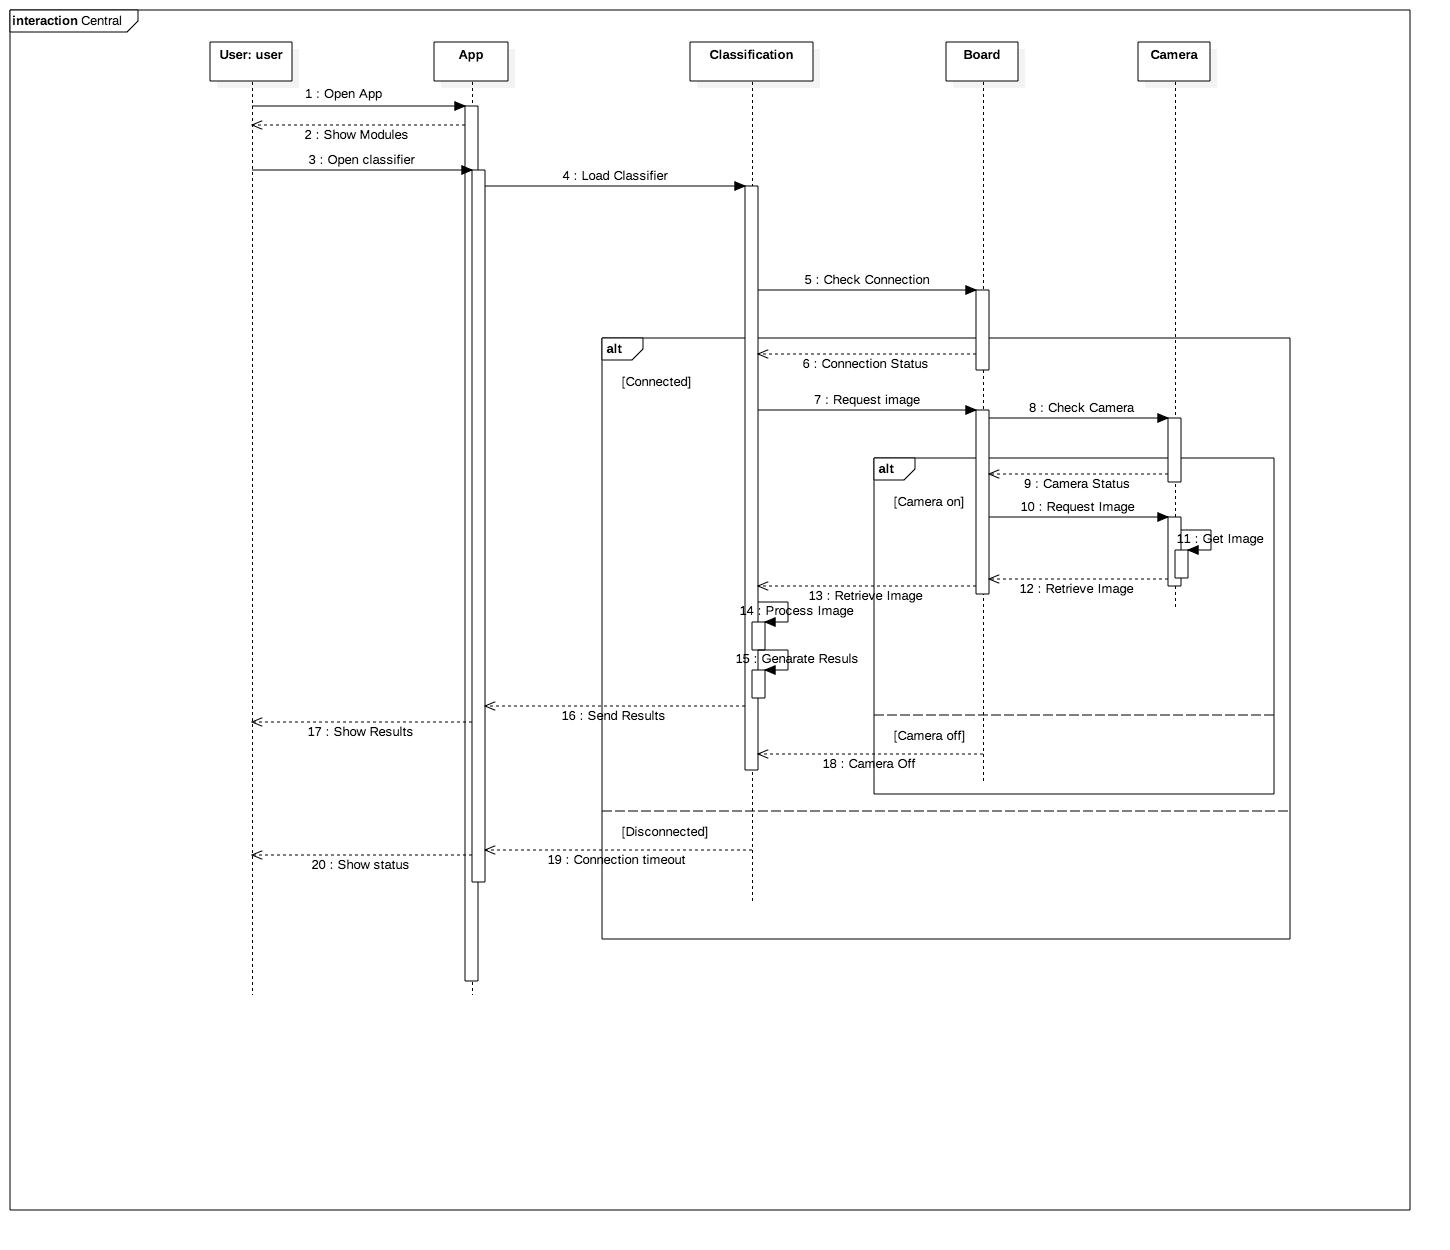
\includegraphics[width = 1\textwidth]			{resources/sequencekraken}
    \end{center}
    \legend{Fonte Própria}
\end{figure}

Detalhando o diagrama \autoref{fig:seqkraken}:
\begin{itemize}
    \item Usuário: o usuário receberá os \textit{feedbacks} através do aplicativo;
    \item Aplicativo: o aplicativo será responsável de entregar as mensagens para o usuário, e manusear a Central (conexão e sensores);
    \item Módulo de Classificação: Consiste em um módulo localizado na aplicação que será responsável por analisar, processar e classificar a imagem;
    \item Boia (Board / Câmera): A Boia que estará conectada à aplicação, onde estarão contidos os sensores e será responsável por adquirir imagens e as enviá-las. 
\end{itemize}


\section{Análise dos dados na central de processamento}

Como ilustra a \autoref{fig:fluxoprocesso}, após a coleta das imagens captados pelos sensores de captura (como câmeras) as imagens serão enviadas através de uma rede \textit{Wireless} para a Central, onde serão processados pelo módulo de Classificação que utilizará \textit{OpenCV} \cite{opencv} para os filtros de pré-processamento afim de melhorar a qualidade da imagem, caso seja necessário, e adequá-las para classificação usando o \textit{Tensorflow}, previamente modelado utilizando \textit{Inception}, para retreinar as últimas camadas da sua rede neural. afim de . 
Após o processamento da imagem, será gerado um relatório sobre os dados processados dessa imagem e o resultado da classificação, exibindo um infográfico mostrando os resultados.


\begin{figure}[ht]
	\centering
    \caption{\label{fig:fluxoprocesso}Fluxo de Processos do Sistema Computacional Proposto}
	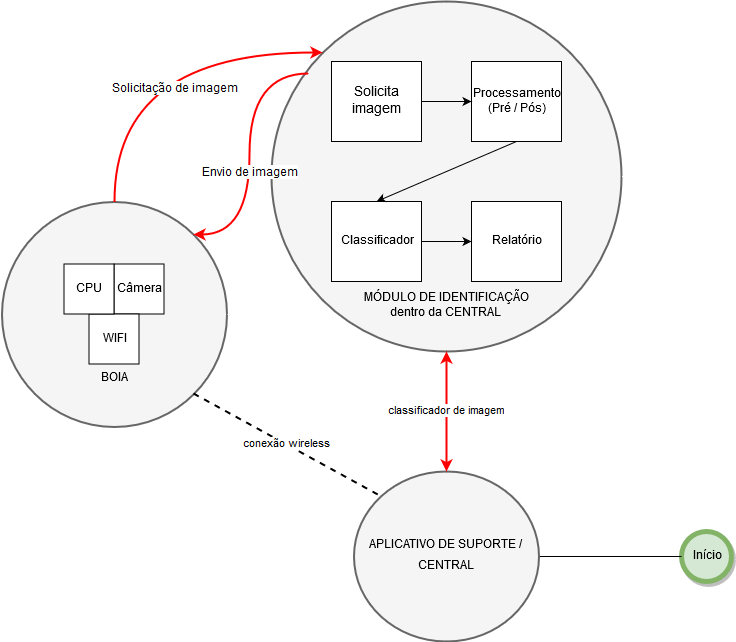
\includegraphics[width = 0.8\textwidth]{resources/fluxo-de-processo.png}
    \legend{Fonte Própria}
\end{figure}

\subsection{Pré processamento}
A etapa de pré-processamento consiste em verificar a qualidade da imagem para decidir se ela, vai passar por certas etapas de processamento para melhorias na imagem, caso a imagem esteja apta a classificação a mesma será enviada  deve ou não ser enviada para o módulo de pré-processamento. Dada a situação onde o ambiente observado não tem suas águas turvas o envio para o módulo de classificação


\begin{figure}[ht]
	\centering
    \caption{\label{fig:bigpic}Fluxo de Pré-processamento}
	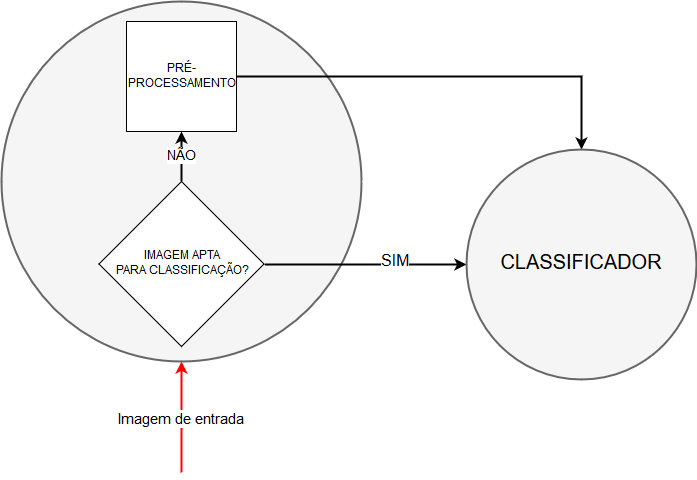
\includegraphics[width = 0.7\textwidth]{resources/fluxoprocessamento.png}
    \legend{Fonte Própria}
\end{figure}

\subsubsection{Filtro Homomórfico}
De acordo com \citeonline{bazeille2006}, o filtro homomórfico pode ser utilizado para corrigir os problemas de iluminação não uniforme e melhorar o contraste da imagem, aprimorando a nitidez da imagem ao mesmo tempo. Um exemplo do resultado da utilização pode ser visto na \autoref{fig:homomo}.

\begin{figure}[ht]
	\centering
    \caption{\label{fig:homomo}Resultado da utilização do filtro homomórfico no método do trabalho de \citeonline{bazeille2006}}
	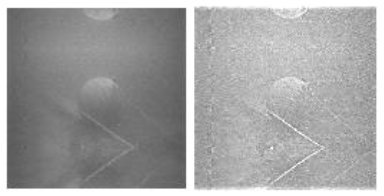
\includegraphics[width = 0.4\textwidth]{resources/homomo1.png}
    \legend{Adaptada de \citeonline{bazeille2006}}
\end{figure}



\subsubsection{Filtro Anisotrópico}
Segundo \citeonline{bazeille2006}, o filtro anisotrópico permite simplificar os atributos da imagem afim de aprimorar a segmentação da mesma, suavizando a imagem em uma área homogênea, preservando as arestas e as melhorando. Esse filtro é utilizado para remover alguns ruídos nas arestas causados pelo filtro homomórfico. Um exemplo da utilização do filtro pode ser visto na \autoref{fig:anisotop}. 

\begin{figure}[ht]
	\centering
    \caption{\label{fig:anisotop}Resultado da utilização do filtro anisotrópico método do trabalho de \citeonline{bazeille2006}}
	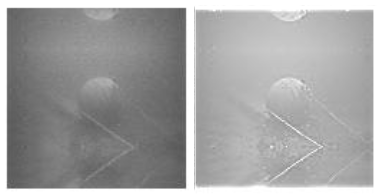
\includegraphics[width = 0.4\textwidth]{resources/anisitrop.png}
    \legend{Adaptada de \citeonline{bazeille2006}}
\end{figure}


%\section{Análise dos sensores}

 %Dada determinada situação onde a água não está com turbidez a utilização de um sensor pode detectar o ambiente e evitar que a central não necessite utilizar os filtros de pré-processamento nas imagens capturadas, melhorando o tempo de classificação.

%Com a possibilidade da adição de extensões à Boia, como sensores de medição de oxigenação da água, a necessidade de analise desses é algo pertinente para o desempenho da boia.



\section{Construção da Boia}

A estrutura da Boia, que é ilustrada na \autoref{fig:blueprint}, que visa baixo custo, utilizará materiais que podem ser encontrados com facilidade, como canos de PVC para a sustentação dos sensores e placas, tendo grande potencial para extensões ou modificações como alterar a estrutura para adicionar outro tipos de motores.

\begin{figure}[ht]
	\centering
    \caption{\label{fig:blueprint} Descrição da construção da Boia.}
	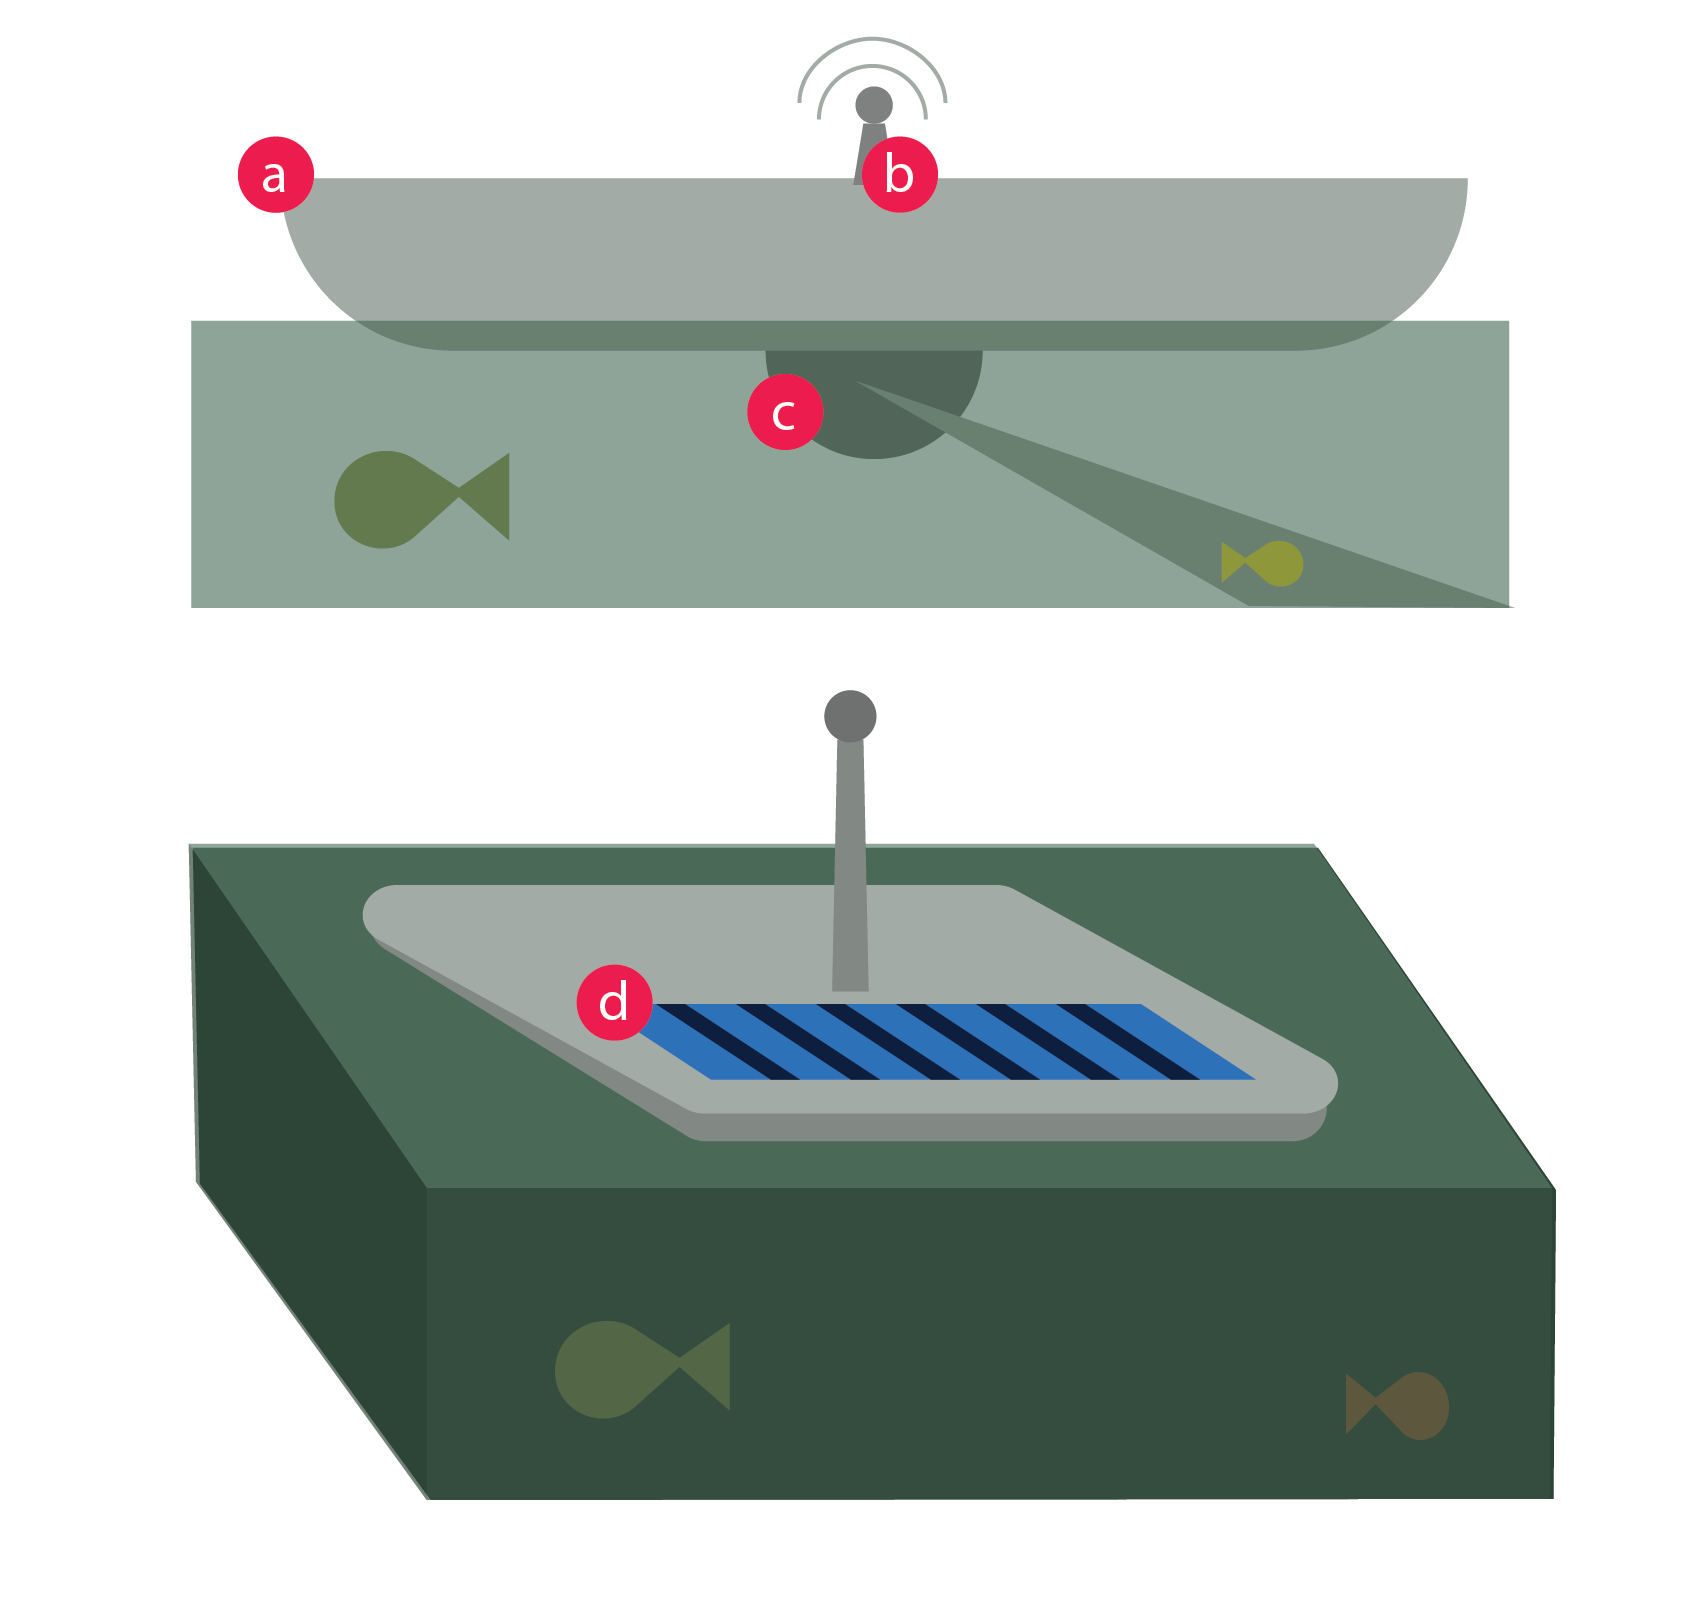
\includegraphics[width = \textwidth]{resources/blueprint.png}
    \legend{Fonte Própria}
\end{figure}

Como ilustra a \autoref{fig:blueprint}, os principais pontos a serem observados na construção da Boia são os seguintes:
\begin{description}
    \item[a.] Corpo da boia: será feito com materiais de baixo custo e de fácil acesso. Está será uma parte importante, uma vez que todos os componentes elétricos da boia estarão armazenados nesse contêiner. Sensores como:
    \begin{itemize}
        \item Placa de circuito integrado (\textit{Single Board Computer}: a placa definida para o projeto será uma variação do \textit{Raspberry Pi zero}\footnote{<https://www.raspberrypi.org/products/raspberry-pi-zero/>}, a \textit{Raspberry Pi zero W} \footnote{<https://www.raspberrypi.org/products/raspberry-pi-zero-w/>}, que por ter conexão \textit{wireless} embutida por padrão, diminuindo os custos com extensão para tal finalidade. 
        \item Sensor de captura óptica (câmera).
    \end{itemize}
    
    \item[b.] Sensor de captura óptica (câmera):  será utilizada a câmera \textit{Raspberry Pi Camera Module v2} \footnote{<https://www.raspberrypi.org/products/camera-module-v2/>}
    \item[c.] Antena: a antena que será utilizada no projeto está embutida no computador de placa única \textit{Raspberry Pi zero W}. 
    \item[d.] Placa Solar: será um painel solar (genérico) que irá alimentar parte do sistema.
\end{description}


%\section{A Boia no futuro}
%Com a possibilidade da adição de extensões à Boia, como sensores de medição de oxigenação da água, a necessidade de analise desses é algo pertinente para o desempenho da boia.

%\section{Identificação de Objetos utilizando openCV}
%O método utilizado para nessa primeira fase de identificações consiste nas seguintes etapas. Como mostra a Figura~\ref{fig:fluxfish} 



%\subsection{Pré-processamento}
%O pré-processamento da imagem é feito com a correção de cores, alterando seu sistema de cores de RGB para BGR como pode ser visto na figura~\ref{fig:fishp1}. 
%\begin{figure}[H]
%	\caption{\label{fig:fishp1} Alteração do sistema de cores para RGB}
%	\centering
%		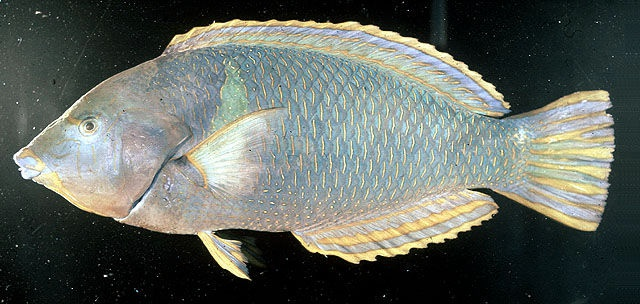
\includegraphics[width = 0.4\textwidth]			{fishes/fish_P1}
 %   \legend{Fonte Própria}
%\end{figure} 
%Para remoção de ruídos um filtro Gaussiano com outra modificação no sistema de cores é aplicado, facilitando a identificação de alguns pontos na imagem. o resultado pode ser visto na figura~\ref{fig:fishp2} 
%\begin{figure}[H]
%	\caption{\label{fig:fishp2} Aplicação de filtro Gaussiano e alteração do sistema de cores para HSV}
%	\centering
%		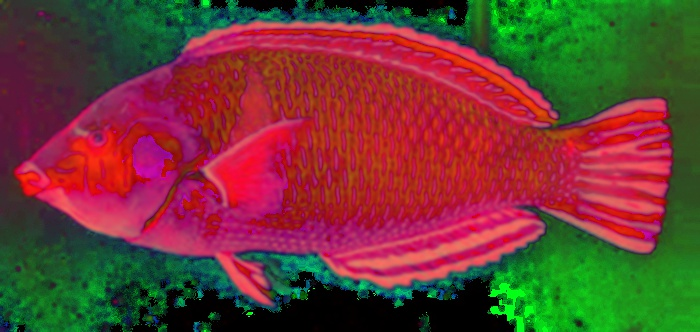
\includegraphics[width = 0.4\textwidth]			{fishes/fish_P2}
 %   \legend{Fonte Própria}
%\end{figure} 

%Em seguida a imagem deve ser livradas de alguns ruídos, assim um filtro gaussiano e conversão do sistema de cores serão aplicados. Resultado na Figura~\ref{fig:fishp2} 


%\subsection{Segmentação e identificação de objetos}
%A máscara de segmentação é baseada nos níveis de cores encontrados na imagem. Dois filtros são criados com espectros de cores diferentes e em seguida mesclados. . o resultado pode ser visto na figura~\ref{fig:fishp3_mask1}, a figura~\ref{fig:fishp5} mostra a exclusão de segmentos não necessários.
%\begin{figure}[H]
%	\caption{\label{fig:fishp3_mask1} Extração das máscaras}
%	\centering
%		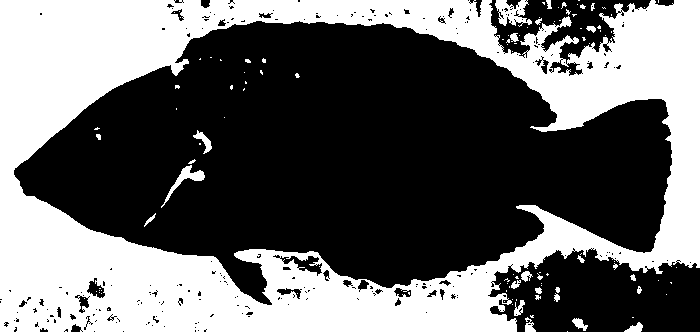
\includegraphics[width = 0.4\textwidth]			{fishes/fish_P3_mask1}
%    \legend{Fonte Própria}
%\end{figure}
%\begin{figure}[ht]
%	\caption{\label{fig:fishp5} Exclusão de segmentos}
%	\centering
%		
\includegraphics[width = 0.4\textwidth]			{fishes/fish_P5_mask_fishes}
 %   \legend{Fonte Própria}
%\end{figure} 

%A identificação de objetos na imagem é realizada através da identificação dos maiores pontos encontrados nas máscaras de segmentação, então esses são circulados, gerando a imagem de saída.
%\begin{figure}[H]
%	\caption{\label{fig:fishp5} Saída}
%	 \centering
%		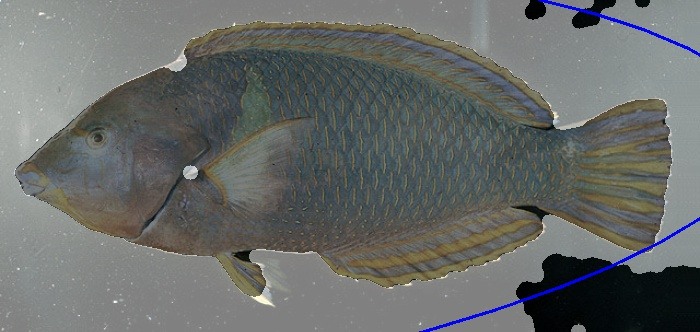
\includegraphics[width = 0.6\textwidth]			{fishes/fish_P7}
%    \legend{Fonte Própria}
%\end{figure}





%\chapter{DISCUSSÃO}

% ----------------------------------------------------------
% Conclusão
% ----------------------------------------------------------
\chapter{CRONOGRAMA}
\label{chapter:consideracoes}

\begin{table}[htbp]
  \centering
  \caption{Cronograma de atividades}
  \label{tab:cronograma}
  \begin{tabularx}{\textwidth}{|X|c|c|c|c|c|}
    \hline
    \textbf{Atividade} & \textbf{Agosto} & \textbf{Setembro} & \textbf{Outubro} & \textbf{Novembro} & \textbf{Dezembro} \\
    \hline
    Criação de modelo formal & \(\times\) & & & & \\
    \hline
    Validação de modelo & \(\times\) & \(\times\)  &  & & \\
    \hline
    Validação de modelo & \(\times\) & \(\times\)  &  & & \\
    \hline
    Validação de modelo & \(\times\) & \(\times\)  &  & & \\
    \hline
    Validação de modelo & \(\times\) & \(\times\)  &  & & \\
   \hline
    Validação de modelo & \(\times\) & \(\times\)  &  & & \\    
    \hline
    Desenvolvimento de software de classificação & & \(\times\) & \(\times\) & \(\times\) & \\
    \hline
    Treinamento do modelo de aprendizado de máquina & & & \(\times\) & &  \\
    \hline
    Testes com o protótipo da prótese & & & \(\times\) & \(\times\) &  \\
    \hline
    Defesa para a banca & & & & & \(\times\)  \\
    \hline
  \end{tabularx}
  %\legend{Fonte: Autor.}
\end{table}

% ----------------------------------------------------------
% Apêndice 1: Revisão Sistemática da Literatura
% ----------------------------------------------------------
\chapter{APÊNDICE 1: REVISÃO SISTEMÁTICA DA LITERATURA}
\section{Revisão sistemática sobre detecção de objetos em ambiente parcialmente observáveis submersos}

  A revisão sistemática da literatura, foi parcialmente executada e foi o ponto de partida do projeto proposto, para encontrar artigos e publicações acadêmicas e industriais relevantes para extração de informações e métodos para identificação e detecção de objetos. A revisão sistemática da literatura utiliza as palavras-chaves relacionadas ao tema e artigos similares ao tema, aliando a formulação de questões de pesquisa para direcionar o estudo da revisão sistemática \citeonline{Kitchenham2009SystematicReview}. Após a seleção das palavras-chaves, uma string de busca foi criada e executada no mecanismo de busca online da editora Elsevier, Scopus. Os resultados foram então processados e filtrados para encontrar artigos relevantes ao tema estudado, por meio de critério de seleção criados para avaliar e selecionar as publicações retornadas. Assim, foram  identificados  trabalhos correlatos e extraídos dados relacionados aos métodos propostos nestes trabalhos.


%     esta seção tem como objetivo apresentar um levantamento bibliográfico baseado na técnica de revisão sistemática, que foi parcialmente realizada, com a execução do primeiro filtro com artigos da base de dados bibliográficos \textit{Scopus}, com o objetivo de identificar e conhecer métodos para detecção de objetos em ambiente parcialmente observáveis em ambiente aquático com alta turbidez, extraindo suas principais características, e avaliando as vantagens e desvantagens de cada abordagem. Um dos principais objetivos desta revisão sistemática é selecionar métodos para serem aplicados neste trabalho.


\subsection{Estruturação das questões de pesquisa}
A \textit{string} de busca foi estruturada seguindo o padrão PICO (\textit{population, intervention, comparison, outcome}) proposto por \citeonline{Kitchenham2007Guidelines2.3}.
Onde:
 \begin{itemize}
 \item  População: Trabalhos publicados em conferências e periódicos que relacionem estudos em ambientes aquáticos submersos.
 \item Intervenção: Relacionam a detecção e reconhecimento de objetos em ambientes aquáticos parcialmente observáveis.
 \item Comparação:  Análise dos métodos e abordagens utilizados para detecção e reconhecimento de objetos nos ambientes estudados.
 \item Resultados: Dado os dados coletados através dos relatos encontrados sobre detecção e reconhecimento de objetos, pretende-se verificar os métodos para avaliar as abordagens encontradas.
 \end{itemize}

A \textit{string} de busca foi desenvolvida em bases nas seguintes características:

População: publicações que fazem referências à estudos em ambientes aquáticos submersos.
\begin{itemize}
\item \textbf{Palavra-Chave:}
"underwater objects" OR “underwater vision” OR “underwater archaeology" OR“underwater images” OR “underwaterimaging” OR "submerged objects" OR “accurate underwater” OR “underwatersites” OR “sonar image enhancement"
\end{itemize}

Intervenção: publicações que relacionam detecção e reconhecimento de objetos em ambientes aquáticos parcialmente observáveis.
\begin{itemize}
\item \textbf{Palavra-Chave:}
“computervisionphotogrammetry” OR “scene contrast” OR"object detection" OR  "object tracking"  OR “object classification” OR “detection and tracking of underwater” OR "object recognition" OR computer vision recognition” OR "object identification" OR  “hidden-object detection” OR "hearlike view"
\end{itemize}

Para a aplicação da revisão sistemática serão definidas alguns itens de planejamento, sendo esses as questões de pesquisas estudadas e o ambiente utilizado. Visando responder as seguintes perguntas:
\begin{itemize}
  \item Q1: Quais são os métodos de detecção de objetos em ambiente submersos com baixa visibilidade? 
  \item Q1.1: Foi desenvolvido e está disponível alguma ferramenta para a aplicação do método?
  \item Q1.2: O método proposto foi gerado a partir da integração com outros?
  \item Q1.3: Qual é a estratégia de execução do método?
  \item Q1.4: Quais foram os resultados positivos ou negativos da validação/experimentação do método?
  \item Q1.5: Quais as limitações do método proposto?
\end{itemize}

\section{Procedimentos de Seleção e Critérios}

A estratégia de busca será aplicada por um pesquisador para identificar as publicações em potencial. A seleção das publicações dar-se-á em 4 etapas:
\begin{enumerate}
\item \textbf{Seleção e catalogação preliminar dos dados coletados:}A seleção preliminar das publicações será feita a partir da aplicação da expressão de busca às fontes selecionadas. Cada publicação será catalogada em um banco de dados criado especificamente para este fim e armazenada em um repositório para análise posterior;
%
\item \textbf{Seleção dos dados relevantes - [1 filtro]:} A seleção preliminar com o uso da expressão de busca não garante que todo o material coletado seja útil no contexto da pesquisa, pois a aplicação das expressões de busca é restrita ao aspecto sintático. Dessa forma, após a identificação das publicações através dos mecanismos de buscas, deve-se ler o título, os resumos/abstracts e as palavras-chave e analisá-los seguindo os critérios de inclusão e exclusão identificados a seguir. Neste momento, poder-se-ia classificar as publicações apenas quanto aos critérios de exclusão, entretanto, para facilitar a análise e reduzir o número de publicações das quais se possam ter dúvidas sobre sua aceitação, deve-se também classificá-las quanto aos critérios de inclusão. Devem ser excluídas as publicações contidas no conjunto preliminar que:
%
	\begin{itemize}
	\item \textbf{CE1-01:} Não serão selecionadas publicações em que as palavras-chave da busca não apareçam no título, resumo e/ou texto da publicação (excluem-se os seguintes campos: as seções de agradecimentos, biografia dos autores, referências bibliográficas e anexas).
    %
	\item \textbf{CE1-02:} Não serão selecionadas publicações em que descrevam e/ou apresentam ‘keynote speeches’, tutoriais, cursos e similares.
    
	\item \textbf{CE1-03:}Não serão selecionadas publicações em que o contexto das palavras-chave utilizadas no artigo leve a crer que a publicação não cita uma abordagem para identificação de objetos submersos em água com baixa visibilidade. 
	\item \textbf{CE1-04:} Não serão selecionadas publicações em que o contexto das palavras-chave utilizadas no artigo leve a crer que a publicação não cita uma abordagem para identificação de objetos submersos em água com baixa visibilidade.
\end{itemize}
\end{enumerate}

Podem ser incluídas apenas as publicações contidas no conjunto preliminar que:
\begin{itemize}
	\item \textbf{CI1-01:}Podem ser selecionadas publicações em que o contexto das palavras-chave utilizadas no artigo leve a crer que a publicação cita uma abordagem para identificação de objetos submersos em água com baixa visibilidade.
	\item \textbf{CI1-02:}Podem ser selecionadas publicações em que o contexto das palavras-chave utilizadas no artigo leve a crer que a publicação cita recomendações de melhoria na utilização de abordagens na identificação de objetos submersos em água com baixa visibilidade
\end{itemize}


\todo[inline]{Figura solta adicionar texto explicando}
\begin{figure}[h]
	\caption{\label{fig:stascorr} Resultados do primeiro filtro.}
	\begin{center}
	    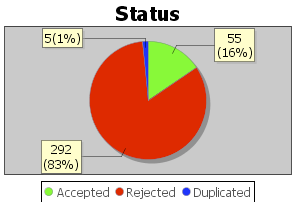
\includegraphics[width=0.4\textwidth]{resources/analisecorre}
	\end{center}
	\legend{Fonte: própria}
\end{figure}

\newpage
% ----------------------------------------------------------
% Referências bibliográficas
% ----------------------------------------------------------
\bibliography{newbib}

%---------------------------------------------------------------------
% INDICE REMISSIVO
%---------------------------------------------------------------------
%\phantompart
\printindex
%---------------------------------------------------------------------

\end{document}
